\documentclass[sigconf]{acmart}

\usepackage{graphicx}
\usepackage{mathtools}
\usepackage{framed}
\usepackage{cleveref}
\usepackage{hyperref}


\copyrightyear{2019}
\acmYear{2019}
\setcopyright{acmlicensed}
\acmConference[HPDC '19]{HPDC '19: International ACM Symposium on High-Performance Parallel and Distributed Computing}{June 24--28, 2019}{Phoenix, AZ}


\begin{document}
\title[Projecting Global Filesystems into Local Containers.]{Projecting Global Filesystems into Local Containers for High-throughput Computing on HPC Resources}

\if 0

Abstract

Intro
- CVMFS & HEP applications
- NERSC/HPC resources
- mismatch, new requirements on HPC

Background and Challenges
- CVMFS requirements
- no FUSE, sudo, etc. on HPC
- Frequent updates to CMVFS
- need for past versions and present
- version consistency issues/mismatch with shared filesystem semantics
- DVMFS

-------------------

Identifying Dependencies
- tracing vs. static analysis
- represent deps. as a set of files -> equivalence between the two approaches
- possibility to include more than requested
- WLCG as testbed for tracing
- overhead of tracing
- sampling ratio for live applications

Projecting a Global FS
- projections vs. images
- SquashFS images vs. Docker, ...
- Shrinkwrap
- quantify image size vs. projection size
- data, metadata, cache costs
- creation costs

--------------------

Managing CVMFS Containers at an HPC Site
- multiple snapshots at different versions
- cost of large number of container images (storage, distribution, etc.)
- extreme cases: massive NERSC image vs. loads of tiny containers
- possibility of replacing an image with an augmented version to serve 2 apps
- tradeoffs in space, creation time, etc.
- online problem: create vs. augment

---------------------

PoC Implementation
- consider (path, ID) to deal with versions
- Jacard distance metric
- group images with common parts
- fast to (approximately) compute
- putting too many disjoint pieces in an image pushes it farther and farther away
- LRU to clean up

Evaluation
- sample workloads
- image vs. projection vs. cache size
- space savings
- image re-use
- construction time
- choice of alpha

----------------------

Conclusion

\fi

\author{Tim Shaffer$^\star$, Nicholas Hazekamp$^\star$, Jakob Blomer$^\dagger$, and Douglas Thain$^\star$}
\email{tshaffe1@nd.edu, nhazekam@nd.edu, jblomer@cern.ch, dthain@nd.edu}
%\orcid{}
\affiliation{%
  \institution{$^\star$ University of Notre Dame   $^\dagger$ European Laboratory for Particle Physics (CERN)}
%  \city{Notre Dame}
%  \state{Indiana}
%  \postcode{46556}
}

%\author{Jakob Blomer}
%\email{jblomer@cern.ch}
%\orcid{}
%\affiliation{%
%  \institution{CERN}
%  \city{Geneva}
%  \country{Switzerland}
%}

\if 0  
\author{Nicholas Hazekamp}
\email{nhazekam@nd.edu}
\orcid{}
\affiliation{%
  \institution{University of Notre Dame}
  \city{Notre Dame}
  \state{Indiana}
  \postcode{46556}
}


\author{Douglas Thain}
\email{dthain@nd.edu}
\orcid{}
\affiliation{%
  \institution{University of Notre Dame}
  \city{Notre Dame}
  \state{Indiana}
  \postcode{46556}
}  
\fi

\renewcommand{\shortauthors}{Shaffer et al.}



\begin{abstract}
Scientific applications often depend on large, complex software repositories containing libraries, tools, and frameworks in multiple versions and platforms to support many researchers.
Such repositories are distributed to hundreds of major computing
facilities around the world using a global filesystem like CVMFS.
However, not all HPC facilities permit execution nodes to
mount and access global network resources, instead encouraging
applications to make use of local filesystems and container
technologies.  In this work, we present a technique for efficiently
\emph{projecting} a global filesystem into local resources.
This consists of creating minimal local containers that meet
the needs of specific jobs, balancing between the extremes
of having many small single-purpose containers and having one
large all-purpose containers.  We evaluate these techniques
using data from production instances of the CVMFS global filesystem
used by a wide variety of scientific collaborations.
\end{abstract}


%
% The CCSXML code is generated by the tool at http://dl.acm.org/ccs.cfm.
% Please copy and paste the code.
%

%
% Keywords. The author(s) should pick words that accurately describe the work being
% presented. Separate the keywords with commas.
\keywords{global filesystem}


\maketitle



\section{Introduction}

Global scientific experiment collaborations like ATLAS, CMS, LIGO,
and LSST make use of hundreds of thousands of cores spread across
many computing facilities around the world in order to achieve the 
massive scale needed to simulate and analyze data from high bandwidth
scientific instruments.  In order to ensure consistency of software
running at many different sites, collaborations establish global
software repositories that publish the tested and trusted versions
of software to be used for production runs.  These repositories
can be quite large, consisting of thousands of software packages
containing millions of files and terabytes of data.  Software
such as CVMFS~\cite{globalfs-cise-2015} is used to distribute
these complex software stacks around the world.

However, not all computing facilities make it easy to access global filesystems at runtime.
In particular, national HPC facilities that are not associated with any
particular experiment often prevent network connections between
individual worker nodes and the outside world, for reasons
of both security and system efficiency.  Such facilities instead
encourage the use of local high performance filesystems and container
technologies to deliver software to individual worker nodes.
To make use of such sites, some mapping between the global
filesystem and the locally available technologies must be provided.

In this paper, we describe the problem of {\bf projecting} a global
filesystem into the resources available at a local HPC facility.
There are two main components to this problem.

First, for a given job, we must have a means of identifying the
subset of the global filesystem that is relevant for the current
execution.  This can be done either by dynamic tracing of the resources
actually used, or by static analysis of its dependency tree.
Using the subset or specification from either method, a projection
then captures the job's software stack.
From this captured software, a minimal container can be
constructed to allow for more efficient storage, transfer, 
and use. We describe Shrinkwrap, 
a tool that produces a minimal software stack 
that can be used to execute the application, or ones closely related.
We analyze the size and make up of global filesystem repositories,
specifically in CVMFS, to show why existing solutions fall short.

Second, for a large number of jobs, we must have a method for
managing the large number of containers that will be created.
If one small container is created for every single job,
site storage will overflow with duplicated data.  On the other
hand, if one large container is constructed to satisfy all
possible jobs, it will overflow constraints at the worker nodes.
To address this, we develop an online algorithm that manages
a shared storage space with multiple containers, choosing to
either create, delete, or merge containers as new requests arrive.
The key parameter ($\alpha$) to this algorithm allows for a
tradeoff between the efficiency of cache storage and container size.

Both techniques are evaluated in light of the properties
of large global filesystems used in production by high
energy physics applications.  In particular, we exploit the
property that many jobs share a small set of frequently-used
dependencies, and have a long tail of infrequently-used dependencies.
We found that our approaches can effectively manage the container images for a continuous stream of submissions with varying software dependencies and versions with less storage overhead than creating a new image per application.
In addition, our results show that applications can still take advantage of precise dependency and version specifications to reduce image creation and transfer overhead compared to simple mirroring.


\begin{figure}
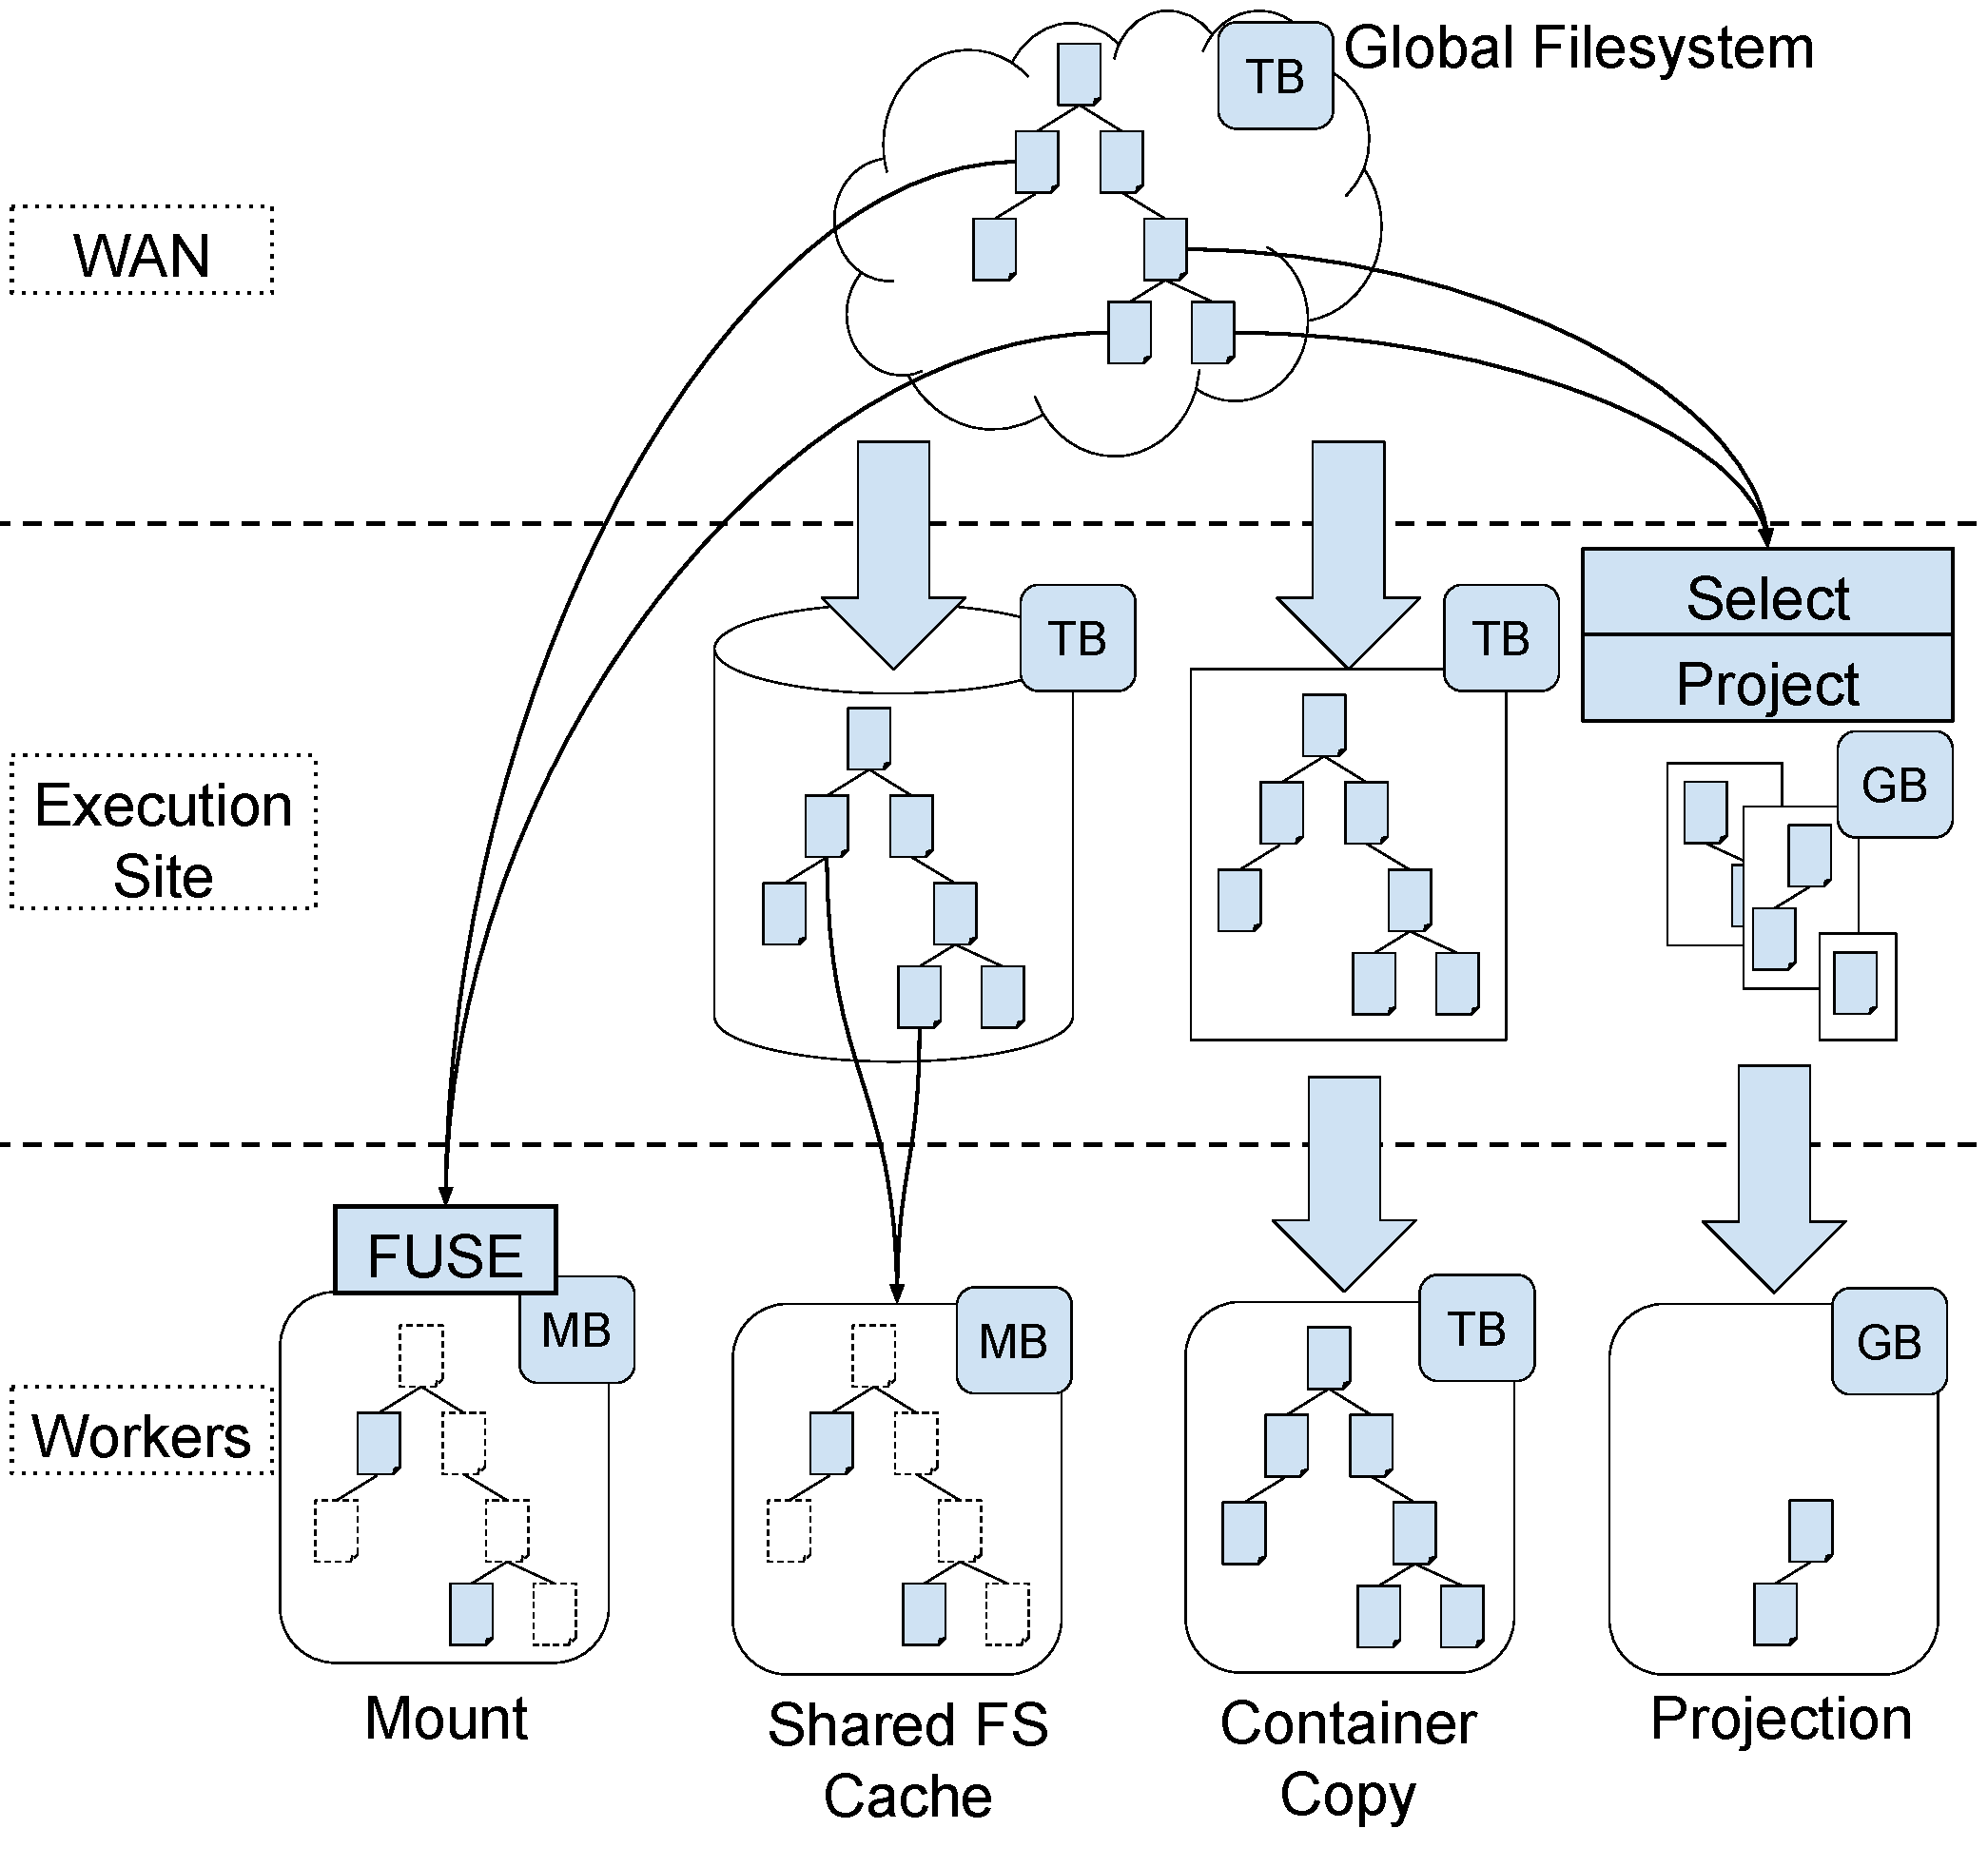
\includegraphics[width=\linewidth]{drawings/methods.pdf}
\caption{Global Filesystem Access Methods}
\label{fig:choices}
\end{figure}

\section{Accessing Global Filesystems}

Modern scientific applications depend upon complex software
repositories that consist of terabytes of data and millions of files.
Unlike ``traditional'' high performance applications that are
single, statically-linked executables, modern applications are
agglomerations of software that consist of high level scripts,
multiple executables written in different languages, support
libraries that may be dynamically linked, and configuration and
data files loaded at runtime.~\cite{casestudy-poster-chep-2015}

In a well-organized project, the necessary software dependencies
are collected together into a global repository that is accessible
from all of the sites that intend to use it.  A common arrangement
is to publish a filesystem that can be mounted from each execution node that intends to use it.  For example, the CVMFS~\cite{globalfs-cise-2015} filesystem is used to publish the software used by all of the major LHC
experiments on hundreds of computing sites around the world.
This requires that the computing site provide the CVMFS software,
and permit worker nodes to access the global network.

\Cref{fig:choices} outlines several broad methods for
accessing such global filesystems.  The simplest
method is to {\bf mount} the filesystem directly from worker
nodes, so that the necessary files can be accessed on demand.
While this is possible at sites that are especially configured
to support the LHC, it is often not possible at other HPC sites
that restrict general network access from worker nodes.
There are many social and technical reasons for these restrictions, but they generally boil down to either security (avoiding intrusions into worker nodes), efficiency (discouraging high value workers from waiting on network access), or configuration (kernel modules are not available to perform the mount.)  As a result, many HPC sites are unable
to use global filesystems of this form.

If that cannot be accomplished, then the next
alternative is to {\bf copy} the entire repository to
a shared parallel or distributed filesystem at the site.
This has the advantage that the filesystem is already
mounted and available at worker nodes.  The entire
repository must be duplicated before it can be used,
regardless of whether an individual job needs it all.
A more subtle problem is that most parallel filesystems are
designed for delivering very large files, and are not at all 
efficient at delivering deep directory trees that
consist of small files and large amounts of metadata,
which describes these repositories as seen in \Cref{fig:cdf}.
When a large number of workers begin to use the software or perform similar metadata operations
simultaneously, the system can collapse from the metadata
load.~\cite{metafs-pdsw-2017,spindle,torrent,exa}

A {\bf container} is often used to reduce the metadata load
on a parallel filesystem.  If a complex software tree is
deployed into a container, the underlying filesystem will
treat the container as a single large file, and be more
efficient at delivering it to many worker nodes simultaneously.
However, if the entire repository (measured in TB) is placed into
the container, it is likely to exceed a number of practical
limits on container size.  Individual worker nodes may have limited
local disk space, or may be entirely diskless.  Even if the
large container fits, it is likely that a given job does not need
\emph{all} of the repository simultaneously, and so it is wasteful
to transfer unneeded data.
This concept is a driving influence on projects like Slacker\cite{194430}.

To have containers of reasonable size, it is necessary to {\bf project}
the required subset of the global repository into a container of reasonable size that can be transferred to each worker node in an
efficient way. Of course, each job that depends upon a repository may need a different subset of the files, so it will be necessary to
maintain multiple container images, within the constraints of available 
storage space.

In this paper, we explore the technique of projecting a global
filesystem into local containers, in order to efficiently use
an HPC facility for a large number of jobs.  This requires striking
a balance between the size of containers, the amount of storage
space used, and the efficiency of data transfer.
We consider two phases of the problem: first, how to describe
and construct a container that serves the needs of a given job,
and second, how to efficiently manage resources when multiple
jobs and multiple containers are required.


\begin{figure}[h]
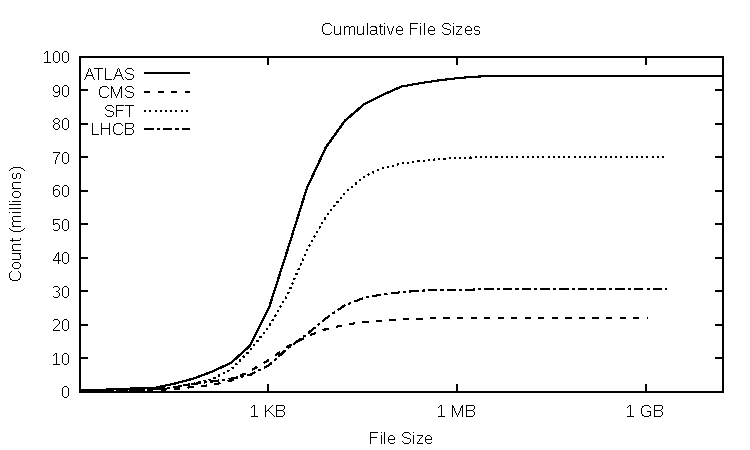
\includegraphics[width=\linewidth]{curated/cdf/cdf.pdf}
\caption{Distribution of file sizes for each repository.}
\label{fig:cdf}
\end{figure}

%%%%%%%%%%%%%%%%%%%%%%%

\section{Creating Projections}

Having defined a projection of a global filesystem as a subset of the filesystem stored locally,
the first step toward creating projections of a global repository is deciding which components to include.
Scientific applications use a wide variety of files, libraries, and packages,
and tend not to respond well to missing components.
When directly mounting a global filesystem or making a local copy,
the entire contents of the filesystem are assumed to be available,
even if any single job only uses a small portion of the total data.
As such, there may not be a convenient and complete description of which pieces of data are required.
Attempting to use a projection based on an incomplete specification leads to potentially intermittent job failures and wasted computing resources.
On the other hand,
including too broad a selection of data in a projection is undesirable as it increases overhead due to extraneous data in the container images.

The simplest way to create a specifications for a projection is manually listing each piece to include.
However, this quickly becomes unfeasible with even a moderate number of software component requirements.
In addition, manual specifications do not necessarily reflect the actual requirements of an application.
Changes to software or simple mistakes can result in incomplete specifications,
and include unnecessary files and data that result in bloated container images.
Manual specifications also practically require consistent, uniform software organization.
This is not a safe assumption within a single repository,
to say nothing of supporting multiple software sources.
This leaves the need for an automated method to create
specifications, such as 
 static analysis or runtime tracing.
To create a comprehensive list of required files and data,
it may be necessary to use a combination of these approaches.

\subsection{Static Dependency Analysis}
    
Static dependency analysis takes advantage of metadata, language, and application-specific knowledge to
discover requirements.
This technique allows applications to be analyzed
prior to running to determine what dependencies from the global filesystem are required.
Static analysis can be informed by several sources of information,
each with varying levels of detail and flexibility.
Language-specific analysis of software components might inspect the \texttt{import} statements in Python or
\texttt{include} directives in C.
These approaches only apply to specific languages or frameworks,
and require some knowledge about how the application is structured.
The software stack used for experiments can also provide information about dependencies in the way it sets up the working environment.
This form of static analysis might involve examining shell scripts for selecting  correct 
software versions, or 
analyzing any number of systems built for 
declaring dependencies, such as 
modules\cite{McLay:2011:BPD:2063348.2063360},
Spack\cite{Gamblin:2015:SPM:2807591.2807623},
VC3-Builder\cite{tovar-ic2e-2018},
or Nix\cite{Dolstra2008NixOSAP},
to determine the configuration.
Additionally it is not uncommon for experiments 
to design and use their own methods such as
SCRAM\cite{DBLP:journals/corr/cs-OH-0306014},
which is used in LHC experiments.
This kind of approach is highly tailored to specific applications or software frameworks and is difficult to generalize to other uses.

In the SFT CVMFS repository, where many of the core research packages at CERN are hosted,
dependency information is included in build metadata associated with each package.
This metadata gives a convenient way to construct a dependency
tree of the entire repository.
We constructed such a dependency tree for the SFT repository to use in the simulations discussed later.
\Cref{fig:picks} gives an indication of the structure and sizes of software components in the repository.
To construct that figure,
we started by repeatedly making random package selections of varying sizes and measuring the total sizes of the selections.
The two lines near the bottom of the graph show these counts and sizes.
Then for each selection of packages,
we used the extracted package metadata to recursively include each package's dependencies.
This recursive resolution simulates the procedure that a program might perform when starting up and loading libraries.
After finding the complete set of dependencies required by each selection,
we plotted the resulting package counts and sizes.
We repeated this procedure 100 times for each choice of specification size,
up to specifications of 1,000 packages.

The plot in \Cref{fig:picks} shows the medians of the resulting measurements.
We observe of course that selection size increases uniformly along the $x$ axis.
The on-disk size of the selections appears to increase proportionally to selection size.
Recursively including the dependencies of these same selections,
however, results in a significant increase in number of packages and size on disk.
For small selections (less than 100~packages),
the complete images with dependencies might contain 5x as many packages as requested,
with storage increasing proportionally.
With larger selections, however,
this increase becomes less prominent.
This non-linear change is the result of the tree structure of the software dependencies.
There are a number of core components that are transitive dependencies of a large number of packages.
These common dependencies are only included once,
so subsequent selections that depend on them do not add them again.
As the number of selections increases,
this curve will approach the total repository size.
Also note that the non-linear increase in size with increasing selection size means that the size of combining two selections of 100 packages (and their dependencies) is not as simple as adding them together.
Due to duplication, we would expect the resulting combined size to be lower,
as if we were choosing 200 packages from the start.



\begin{figure}
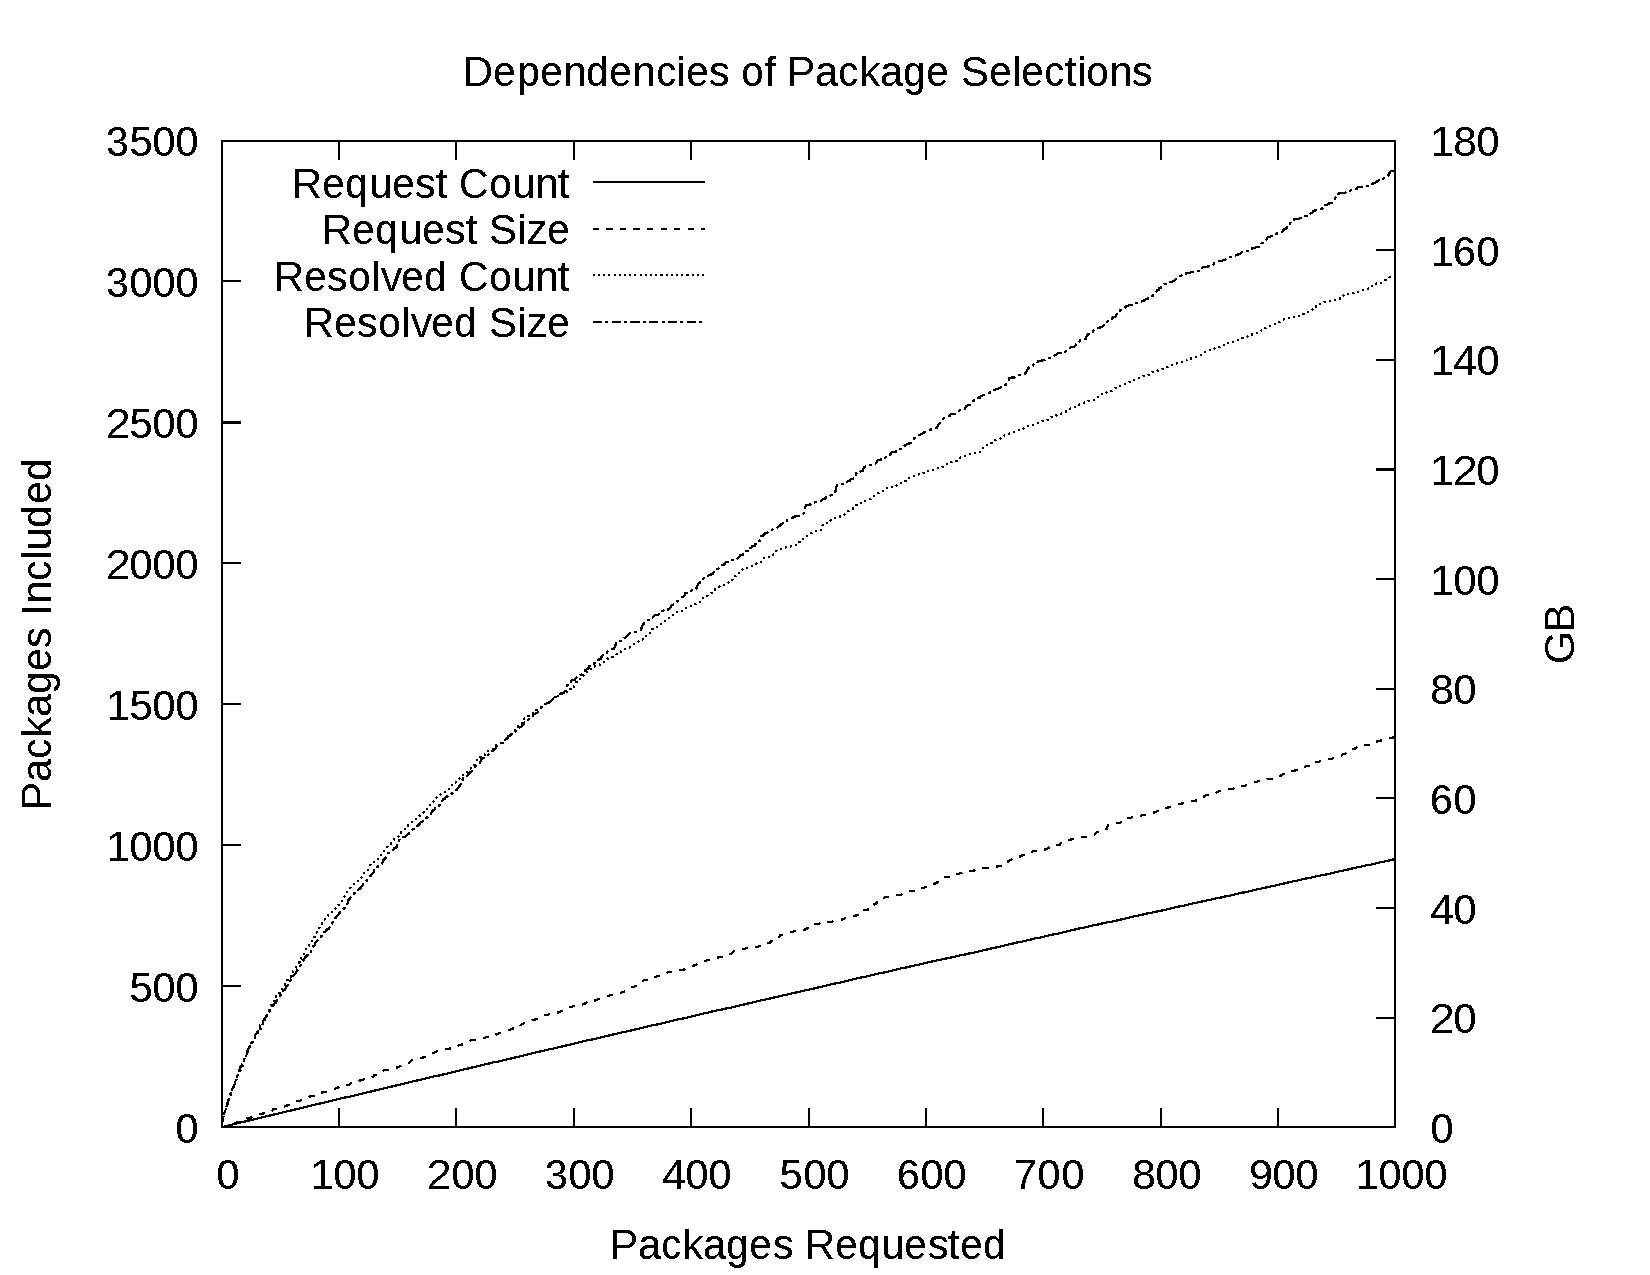
\includegraphics[width=\linewidth]{curated/closure/closure.pdf}
\caption{Difference in number of packages and size when accounting for dependency based closure in selection.}
\label{fig:picks}
\if 0
you get more than you ask for
smaller requirements have relatively large responses
non-linear, so bigger ones have more duplicates
approaches repositories size in limit
merging is subject to drop-off(more duplication)
\fi
\end{figure}

\if 0
\begin{figure}
    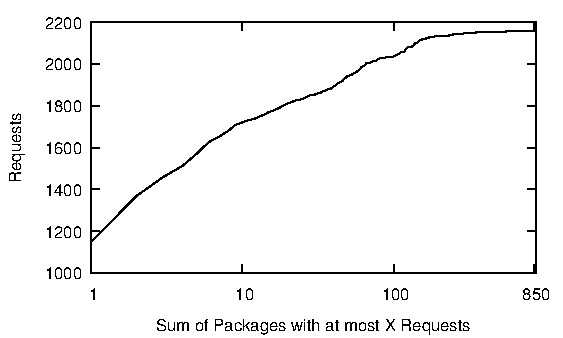
\includegraphics[width=\linewidth]{curated/lxplus_dist/usage_distribution_cdf.pdf}
    \caption{Usage distribution pulled from CERN LXPlus interactive machines.}
    \label{fig:usage_distribution}
\end{figure}

spread across everyone, lot of commonality/overlap
few with very high usage, very large number of rarely used
lot not observed
\fi



\subsection{Runtime Tracing}
Rather than examining the static data and metadata associated with a software collection,
we can use runtime tracing to identify the dependencies used during a particular job.
This trace of a sample job gives an exact listing of the files used,
which is more accurate and reliable than handwritten listings.
A potential drawback is that tracing does not determine every possible dependency,
only those used during a particular sample.
This can be problematic for non-deterministic or data-dependent workloads.
As such, it is preferable to trace a number of jobs.
Since scientific applications routinely consist of thousands
to millions of jobs, sampling a small subset
can provide good software coverage with little
additional overhead. % the computation is still used
The performance cost of creating these traces is
dependant on the method used.
A tracer library based on \texttt{LD\_PRELOAD} can be extremely lightweight but require modification to the execution environment.
More invasive methods include using Parrot to track used files, % I think parrot was mentioned previously
or building the tracing as part of the application.

An important advantage of runtime tracing techniques is that they can function reliably across multiple languages and applications.
This makes it is easier to automate sampling of unknown applications without assistance from each user,
since there is no need to delve in to the particular application
design and configuration.

As part of this work, runtime tracing was introduced
into the CVMFS FUSE client and can be activated for sampling.
When tracing an application,
each filesystem access is recorded and added to the trace log.
Tracing through CVMFS is convenient as it does not require changes to applications,
and the FUSE client is widely deployed across compute sites.
Users have the option of collecting this trace information themselves by re-configuring the client.
For applications running on the Worldwide LHC Computing Grid~(WLCG),
it would also be possible to instrument a fraction of runs to build a profile of a given task.
This introduces the possibility of automatically collecting traces to use when porting applications to more restrictive environments.
    
\subsection{Building Projections}


\begin{table}
\begin{center}
\begin{tabular}{|c|r r r|}
\hline
Repository & Total Size & inode Count & Deduplicated \\
 & (GB) & (K) & Data (GB) \\ \hline
alice & 3,981 & 27,322 & 2,099 \\
atlas & 6,195 & 120,599 & 3,761 \\
%boss & 120 & 2,418 & 72\\
cms & 582 & 26,225 & *2,243\\
%geant4 & 298 & 7,128 & 68 \\
grid & 31 & 714 & 19 \\
lhcb & 2,135 & 33,737 & 368,070 \\
%na61 & 5 & 26 & 2 \\
sft & 3,997 & 128,609 & 2,017 \\ 
 \hline
\end{tabular}
\caption{CVMFS repository sizes.}
\label{tab:repo-sizes}
{\small \it This table shows the size, number of inodes (rounded to nearest thousand), and the amount
of duplicate data that is eliminated using CVMFS.}
\end{center}
\end{table}

Several existing utilities such as UnCVMFS and 
rsync have been used to create projections of CVMFS.
UnCVMFS is a utility that projects an entire
CVMFS repository, at a set revision, into the local
filesystem. 
UnCVMFS utilizes CVMFS's efficient, content-based storage
to deduplicate the underlying data, but requires
entire repositories to be projected.
When used with several repositories for large projects,
unCVMFS can easily consume terabytes of disk space for a single projection.
In addition, it is expensive to update to different revisions of a repository using unCVMFS,
which can create headaches when working with different experiments and analyses that may have conflicting revision requirements.

Rsync allows for file lists to specify and download
subsets of CMVFS repositories, but because it
was designed for general filesystem synchronization
rsync is not aware of the internal organization of CVMFS.
This leads to slow operations and unnecessary duplication of data,
especially when creating multiple projections.

We built the CVMFS Shrinkwrap utility to create projections of CVMFS with better efficiency and finer control than is possible either unCVMFS or rsync individually.
Shrinkwrap uses the CVMFS's client interface to
create and update CVMFS projections.
Shrinkwrap uses a CVMFS configuration to specify the
revision of the repository, a file-specification list
to determine the repository subset to project, and
deduplicates the data in a user specified location.
Shrinkwrap can be configured to share the data
repository between several repositories and even
projections of the same repositories.
This allows for multiple realized projections
to coexist, with the desired projection
mounted for use.
In \Cref{figure:shrinkwrap-arch} you can see an outline
of the design of the Shrinkwrap utility.

\begin{figure}[h]
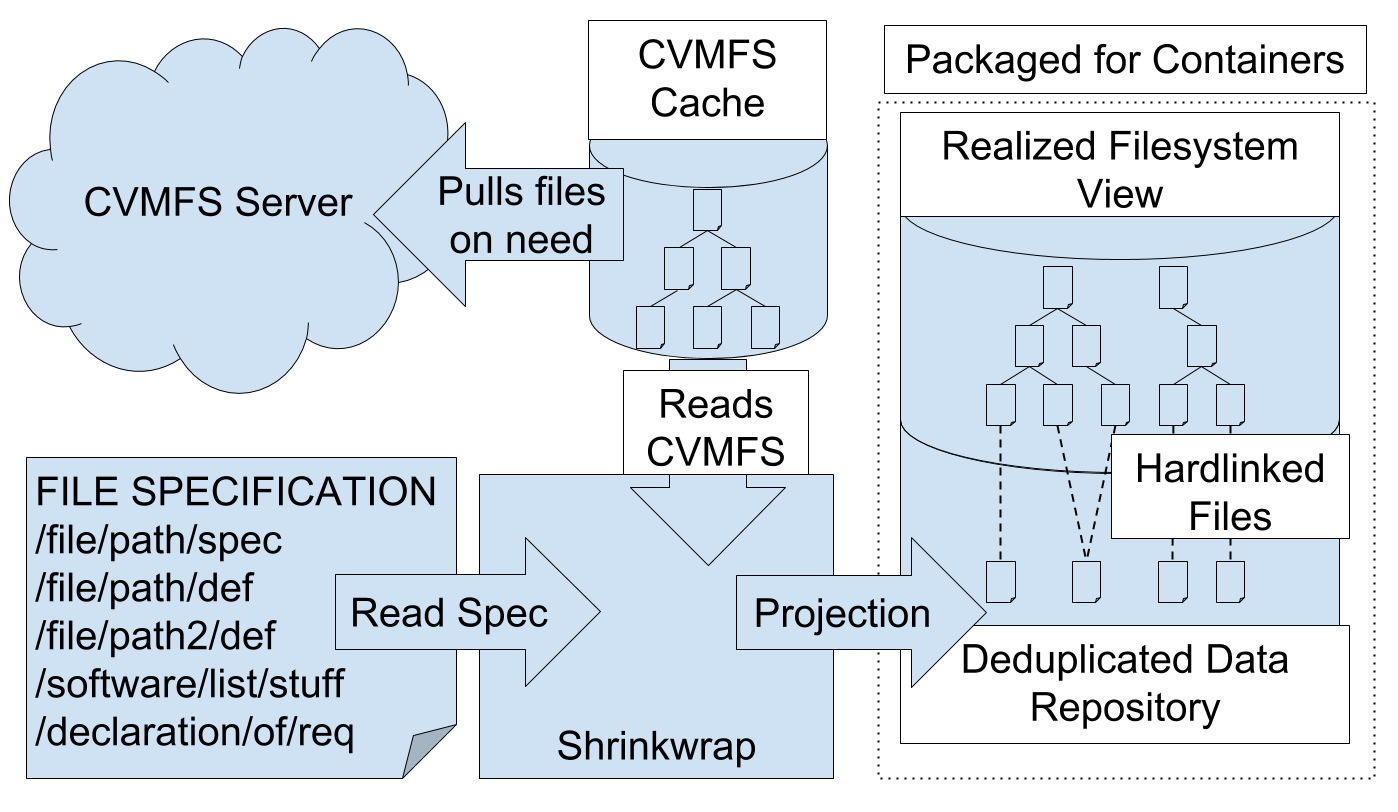
\includegraphics[width=\columnwidth]{drawings/shrinkwrap-structure.png}
\caption{Operation of Shrinkwrap}
\label{figure:shrinkwrap-arch}
\end{figure}


\subsection{Building Container Images}

After creating a file specification for an application and projecting the required data from the global filesystem,
the next step is to create a container image to be used locally.
The simplest approach for automatically projecting container images is to create a suitable image on each batch job submission.
Assuming a file specification has already been created,
it is passed to Shrinkwrap to create the requested projection,
which is then processed into a container image,
for example using \texttt{mksquashfs}.
Unfortunately, this solution is very wasteful of computing time and storage space.
Even a minimal image consisting of a precise set of required libraries and frameworks ranges in the tens of gigabytes,
depending on the application.
A full copy of a repository would consume multiple terabytes of disk space and take the majority of a day to create.
In addition, image creation must be completed before any actual processing occurs,
i.e.\ there is no way to start with a partial image that supports the first steps of a pipeline and finish building the image as the pipeline runs.
There is also the cost of transferring and storing freshly created images on any nodes that will use them,
further delaying job dispatch and increasing load on the network and storage infrastructure.

The disk I/O alone required to create even a targeted image is likely to take more time than a short simulation or analysis job.
Thus a simple performance improvement is to re-use previously created container images for multiple jobs.
A single experiment submitting computational tasks is likely to request the same projection,
at least for jobs submitted around the same time.
It is straightforward to check for exact equality between projections as long as the system tracks the set of files that went into their creation.
If there are few CVMFS users at a site,
this method could be sufficient.
Users simply maintain image collections for use with their jobs.

Unfortunately, a number of real-world usage patterns are poorly handled by this approach.
A small change to a projection,
such as adding a library or updating dependencies,
results in the creation of a second, unrelated image.
Even a small change such as removing an unnecessary documentation file results in a completely new container image.
This is a manageable nuisance when manually testing or developing a system,
but would present a problem for a system managing images automatically and receiving updated specifications over time from tracing jobs.

In addition to unnecessary duplication for a single user/application,
there is also significant duplication across multiple users.
In the simulation and analysis pipelines at CERN,
a number of large components (such as ROOT) are used nearly universally.
These components provide basic functionality and infrastructure that each experiment's software stack builds upon.
Moreover, these same common infrastructure components must be included regardless of user or application.
Thus even if every user of the system only creates a single container image,
there is a duplicate copy of all such common infrastructure components for each user.
This is problematic if we would like to design a system that can support many users at a site.

These two sources of duplication tend to compound each other,
leading us to conclude that a more sophisticated approach is necessary to work with realistically-provisioned workers and system infrastructure.
These issues are fundamentally related to unnecessary duplication of data among container images.
The same types of issues motivate the use of dynamic libraries for everyday applications.
With statically linked executables,
each application includes a complete set of required libraries.
While very stable and reliable,
OS distributions prefer to use dynamic linking.
This allows applications to share a single copy of each library,
so that foundational components such as libc are not copied into every executable,
and so that updates and changes to the set of installed packages do not require rebuilding the entire system.
For this approach to work,
package maintainers must arrange all software packages in the system to ensure compatibility,
and the OS distribution must set policies for system organization, update procedures, etc.
Container images here function similarly to statically linked executables,
but since multiple complete OS distributions are stored within CVMFS,
and since we are dealing with multi-terabyte repositories and entire frameworks and software stacks rather than individual OS libraries,
the scale involved is of course larger.
In the case of CVMFS, there is no notion of a ``package mainainer'' or central authority over all software.
Each experiment manages its own software repository as it chooses,
with some components and repositories shared between multiple applications.
Since we would like to be able to automatically handle existing applications that are not designed with central management in mind,
we must instead look to other approaches for dealing with data duplication as a result of copying data into container images.

\section{Managing Projected Images}

The representation of projections as disk images is problematic for deduplicating data.
Internally, Shrinkwrap uses hard links to a common data store so that a single file is only stored once across all projections in the system.
On creating disk images, however,
these links are broken.
Each disk image must contain a complete copy of all data,
so that a file must be included (and take up space) in every image that includes it.
Docker's solution is to build container from layers of archives that can be reused.
Docker layers are explicitly defined when writing a Dockerfile.
With CVMFS, however, there is no existing layer-like organization or universal rule that could derive layers for existing applicaions.
Working with layers defined from the outset is also a poor fit if we would like to support partial, gradually improved information from traces.
We therefore desire some sort of deduplication that can be applied for existing applications to an assortment of container images after creation.

To develop a deduplication strategy,
we started with some observations about the projection and image properties.
For ``large'' images,
there is limited opportunity for deduplication.
Each large image is a fairly complete copy of a particular repository.
While there is bound to be some overlap between versions of the same repository,
an updated image will contain a large number of updated software components,
making a ``deduplicated'' between two versions significantly larger than either individually.
There are also likely to be some conflicts in the filesystem if software components re-use the same paths for different files between versions.
This case is akin to combining RHEL~6 and RHEL~7 in an attempt to save space.
While there are similarities between the two,
the significant changes and conflicts make this a poor strategy.
Thus for our strategy we would like to avoid ``deduplicating'' images that have large non-overlapping portions.

Likewise, there is little reason to attempt to deduplicate large images built from different repositories.
Such images would have little to no overlap,
so the only benefit to combining the two would be reducing the number of images by one.
This comes at the cost of needlessly storing and transferring the unused half.
This case is akin to bundling a complete Debian installation alongside RHEL.
Our deduplication strategy should only take effect for images with significant overlap.

It is also undesirable to combine images of drastically different size.
As an example, suppose a user creates a small projection as a subset of a repository for running a specific application.
This small image overlaps completely with a large image of the whole repository,
and there is likely no conflict.
Automatically combining the large and small image, however,
can have unintended consequences.
Small, tailored images minimize transfer and storage overhead,
and can be important for operating at scale.
It is therefore unwise to surprise users by suddenly making their container images several orders of magnitude larger.
This is akin to distributing a library exclusively by placing it within a disk image of a Debian installation.
We would therefore like to attempt deduplication only for
{\bf similarly-sized images, with large overlap and with no conflicting paths}.


\subsection{Measuring Similarity Between Projections}

    Having set out the conditions under which to consider deduplicating projected images,
we are in a position to define a metric to quantify the similarity between images.
This would allow us to identify projections that are ``close'' (for some definition of close) as candidates for optimization.
We chose the Jaccard distance under appropriate choice of set elements as it conveniently satisfies the desired qualities set out above,
and is very well used and studied.
In our case, we must describe a container image as consisting of a set of (path, content hash) tuples.
CVMFS already stores files by the hashes of their contents,
so this information is readily available.
Considering both the file names and contents is important as CVMFS allows for updates to file contents over time.
We chose fine-grained tracking of file contents rather than simply recording the version of the CVMFS repository to afford additional opportunities for dedupliaction.
Since each update to a repository does not change the contents of every (or even the majority of) files,
data from multiple repository versions may well be able to coexist in a single container image.

For two sets $A$ and $B$,
the Jaccard distance $d_j$ is defined as follows.
\[
d_j(A, B) = 1 - \frac{|A \cap B|}{|A \cup B|} = \frac{|A \cup B| - |A \cap B|}{|A \cup B|}
\]


For this application in particular,
the Jaccard distance captures several desirable properties of projections.
In the case of two projections that differ only by one file,
the Jaccard distance will be small.
Likewise for a pair of projections with nothing in common,
the distance will be high.
And since the Jaccard distance is a proper metric,
related projections will tend to occur in clusters;
if two projections are both found to be extremely close to a third projection,
we can conclude that the two are themselves close by the triangle inequality.
Other choices of metric may well be viable,
but we found the Jaccard distance to be both well-studied and amenable to efficient approximate implementation.
As described in the following,
we used MinHash~\cite{minhash} as a constant-time approximation of the Jaccard metric as a first pass at selecting similar images.
Such an approximation is important in practice due to the sizes of the data involved;
metadata listings alone (not including any file data) consumed multiple gigibytes of storage in some of the container images we evaluated.

\subsection{Container Management as an Online Problem}

\begin{figure}
\centering
\fbox{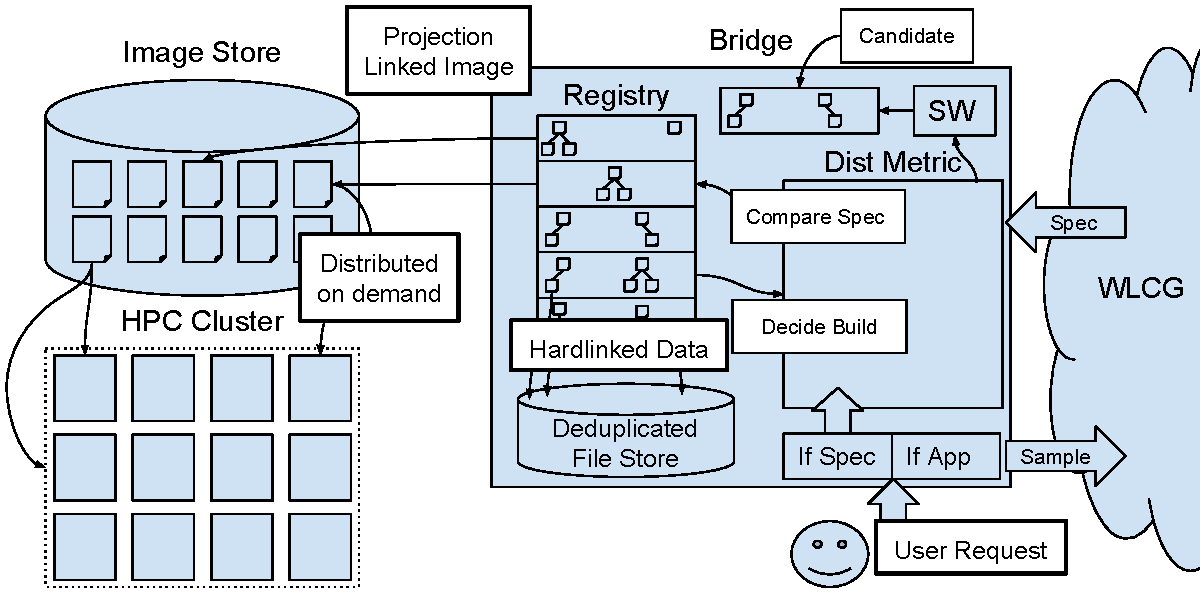
\includegraphics[width=\linewidth]{drawings/system_architecture.pdf}}
\caption{Architecture of a Site-wide Image Management System}
\label{figure:sys-arch}
\end{figure}

 Combining the tools and techniques introduced so far,
we are now ready to address the central problem in managing projected images as a site-wide service.
Rather than relying on administrators to manually manage images,
we must define a method for making a decision online as to how to efficiently satisfy the dependency requirements for submitted jobs.
Our method must be suitable for inclusion either in individual researchers' workflows or as part of the setup for batch job scheduling, and must be efficient in terms of both computation time and storage space.
Our approach will be to track similarity between projections and allow existing images to be augmented rather than creating new ones for each job request.
\Cref{figure:sys-arch} gives an overview of the structure of this system.

Our method will be based around a cache of container images used to satisfy job specifications.
Upon receiving a request for a projection,
we first hash the new projection according to the MinHash algorithm.
We always store the hash values computed for every projection we build to allow for fast clustering.
Next, we use MinHash to approximate the Jaccard distance between the new projection and all projections previously built.
This computed distance can be cached to ensure that we estimate the distance between each pair of images only once.
Since comparisons using MinHash take constant time for a given probability bound independent of the size of the sets involved,
we can quickly identify cached projections that are similar to the new request.

To decide if two projections are ``close enough'',
we define the parameter $\alpha$ as the maximal Jaccard distance between closely related projections.
Since Jaccard distance is by definition between zero and one,
$\alpha$ must be in the same range.
This $\alpha$ parameter is something like the ``globbiness'' of the system.
Small choice of $\alpha$ requires that projections be extremely close before considering them for merging.
In the extreme case with $\alpha = 0$,
only \emph{identical} images will be considered close so no images will be merged.
This results in a larger number of independent images.
Choosing $\alpha$ to be larger makes it more likely for images to be considered similar and merged.
This results in more augmented images that serve multiple tasks.
In the extreme case of $\alpha = 1$,
\emph{every} pair of images is considered close and merged if possible.
This results in large container images that have accumulated many projections.
We explore tradeoffs in terms of efficiency and performance when choosing $\alpha$ in \Cref{sec:eval}.

Having selected a set of candidate projections that are close enough to the new request,
we next check each in turn to find either a superset of the requested projection or one without version incompatibilities.
We first sort the list of candidate images by Jaccard distance.
This ensures that our system prioritizes candidates that are similar in size to the requested image.
In the case of finding a superset,
we can simply use the corresponding cached container image.
Presumably this superset was created by the merging process below,
so we are done.
Otherwise, we continue to look for a compatible projection
Two projections are incompatible if they both include the same path but point to different data.
This situation can arise if for example a library in CVMFS is updated in place.
Old and new projections would include an identical filesystem path,
but the new version would have different contents.
This situation can arise in more subtle ways,
for example with symlinks controlled by environment variables.
Since projections of CVMFS must statically resolve such links,
incompatibilities can arise despite paths appearing compatible under CVMFS.
Any candidate projections that are incompatible with the new request are removed from further consideration.

If no compatible projections were found among the candidates,
we create a container image for the projection as requested and add it to the cache.
Otherwise, on finding a compatible cached projection the next step is to augment it with the contents of the new request.
We choose the first compatible image from the list of candidates for merging,
i.e.\ the compatible image with the smallest Jaccard distance,
which again prioritizes images that are similar in size and contents.
We can use Shrinkwrap to efficiently augment projections to include new or updated contents.
Next, we build a container image based on the newly updated projection.
The computational cost of this step could become high since we are creating larger combined projections.
Appropriate choice of $\alpha$, however,
bounds the distance between the combined projections such that the cost of creating the augmented container is arbitrarily close to cost of simply fulfilling the original request.
Since the augmented projection is the union of two different projections,
it can be used for jobs requiring either.
Thus on merging, the augmented projection can replace the existing image,
so that the net increase in storage space comes only from the newly added files.
Since a single augmented image now serves two different batch job submissions,
we reduce duplication in the cache by avoiding making two copies of the common files and data.

One potential issue with this merging strategy is that there is no way to prevent poor merging decisions.
In the case of a one-off submission,
the system might merge an existing, frequently used image.
This is not problematic for the one-off job itself,
but increases overhead for subsequent jobs.
The original, frequently used image would increase in size with no additional benefit to other tasks.
Images might become ``bloated'' in this way,
accumulating infrequently used dependencies and increasing overhead indefinitely for future tasks.
The Jaccard distance metric gives a natural way to capture and quantify this effect.
As an image becomes bloated due to repeated merges,
its distance from every individual request increases.
After sufficient growth,
the image will become too far from any request to even be considered.
Without regular use,
the bloated image will eventually be removed in LRU order.
Choice of $\alpha$ allows an upper limit on the amount of useless bloat in images.   

\subsection{Simulating Projections}

\if 0
Based on correspondence with researchers,
we made some general observations about the behaviors and requirements of applications we need to support.
First, there are some components such as ROOT that serve as common, foundational components to almost every other simulation and analysis stack.
These core components are often stored separately from the rest of the software collections available in CVMFS.
Second, there are shared components such as setup scripts, configuration files, and calibration or condition data (required to interpret readings from detectors) that are also nearly universally required but are more particular to a given experiment or group.
Finally, there is the collection of software maintained by each experiment.
Software collections may contain multiple copies of the same software for different architectures and versions.
A single analysis job does not use the majority of the available software.
There is some overlap among these categories of software,
for example some software components are widely enough used to be considered core components,
and usage and availability of components varies over time.
\fi

    Since there are currently few regular CVMFS on HPC users,
we decided to simulate the activity of users requesting container images.
We decided to simulate at the granularity of packages rather than individual files,
because this results in more robust container images.
As mentioned previously,
fine-grained tracing runs the risk of leaving out important dependencies.
In addition, working only based on the properties of individual files ignores the structure inherent in software collections.
Looking only at the properties of individual files,
Figure~\ref{fig:cdf} shows cumulative distributions for file sizes in several of the largest and most active CVMFS repository.
The repository vary in scale,
but all show similar usage patterns.
We see that across all repositories,
the majority of files are small (between 1~KB and 1~MB).
The repositories do contain, however,
a small number of large files.
This fits our expectation that the CVMFS repositories primarily contain software.
Most individual files are small,
but the repository size is defined by the large number of packages in the software collection.

We tested two schemes for generating image requests, taking into account the properties of the software collections,
as well as recorded user activity patterns.
We also generated images via a uniform random scheme for comparison.
We consulted with the developers of CVMFS,
as well as HEP researchers at the University of Notre Dame collaborating with CERN to determine how current users interact with CVMFS.
Since CVMFS is not currently widely deployed on HPC resources,
the prospective user base for our container management system is limited.
We were, however, informed of some researchers and groups experimenting with static mirrors of CVMFS for container images,
including projects at NERSC and Stanford University,
with one of the setups available publicly at \url{https://github.com/wyang007/atlas-fat-container}.
    
 We use these observations about the structure and behavior of applications on CVMFS to build a simplified simulation taking into account dependency requirements for evaluating our container image management scheme.
For the purpose of simulation,
we assume that the requirements of a job are given as discrete components or collections of files.
While Shrinkwrap can operate at the granularity of individual files,
both static analysis and runtime tracing produce file collections to include.
We are intentionally somewhat vague here to allow for both explicitly defined software components and tracing outputs.
We examined the software collections available in the SFT repository and constructed a DAG of dependencies among the packages.
The currently available software collection in the SFT repository consists of 9660~packages,
where a program or library typically provides packages for multiple versions and configurations.
When building a projection,
we recursively include dependencies of requested software.
This more closely approximates the structures of actual container images,
while still allowing for randomly selected package requests.
For each simulated image request,
we chose a random selection of packages (either uniform random selection or subject to the process below)
and then added the closure of the package dependencies.
This first image simulation scheme captures the structure inherent in the software collection,
in that packages in addition to those requested are automatically included so as to ensure a functional image.
The initial selection of packages,
however, is simply uniformly random.
This is not necessarily realistic
so we also took usage patterns into account.

We assumed that certain components are included in most container images,
while other components are relatively rarely used.
While multiple versions and variations might exist,
these components have a very high likelihood of appearing in every container image.
These components correspond to the core components, setup scripts, calibration data, etc.\ described previously.
For the purposes of simulation,
we would like to see these components in a large proportion of jobs across all users and experiments.

We obtained CVMFS usage logs from frontend nodes at CERN,
which give rough usage frequencies of the packages in the SFT repository.
To generate simulated container requests,
we made random package selections subject to the observed distribution of package use.
Many packages in the repository were not observed being used at all,
so we added a small, non-zero probability of selecting packages lacking usage data.
We applied this technique in combination with the package dependency graph,
so that images contained a weighted random core selection along with any dependent packages.
This second image simulation scheme takes into account the dependency structure of the repository as well as usage patterns observed in the wild.

As a base for comparison,
we also generated simulated images consisting of packages chosen in a uniform random way.
To ensure that total size (or at least total number of packages)
is comparable to images generated by the previous two methods,
for this approach we started with an image request generated via the first scheme discussed
(uniform random core selection with dependencies added).
We considered only the number of software packages in the resulting image,
and then chose the same number of packages uniformly randomly from the entire repository,
ignoring usage information and package dependencies.
while images generated in this way are not particularly realistic,
they will be useful for evaluating image management schemes.
By comparing results with random images to those with the previous two image generation schemes,
we can compare the general case of containers as collections of arbitrary data to the specific focus of this work,
i.e.\ containers with selections of experimental software.   

\begin{figure}
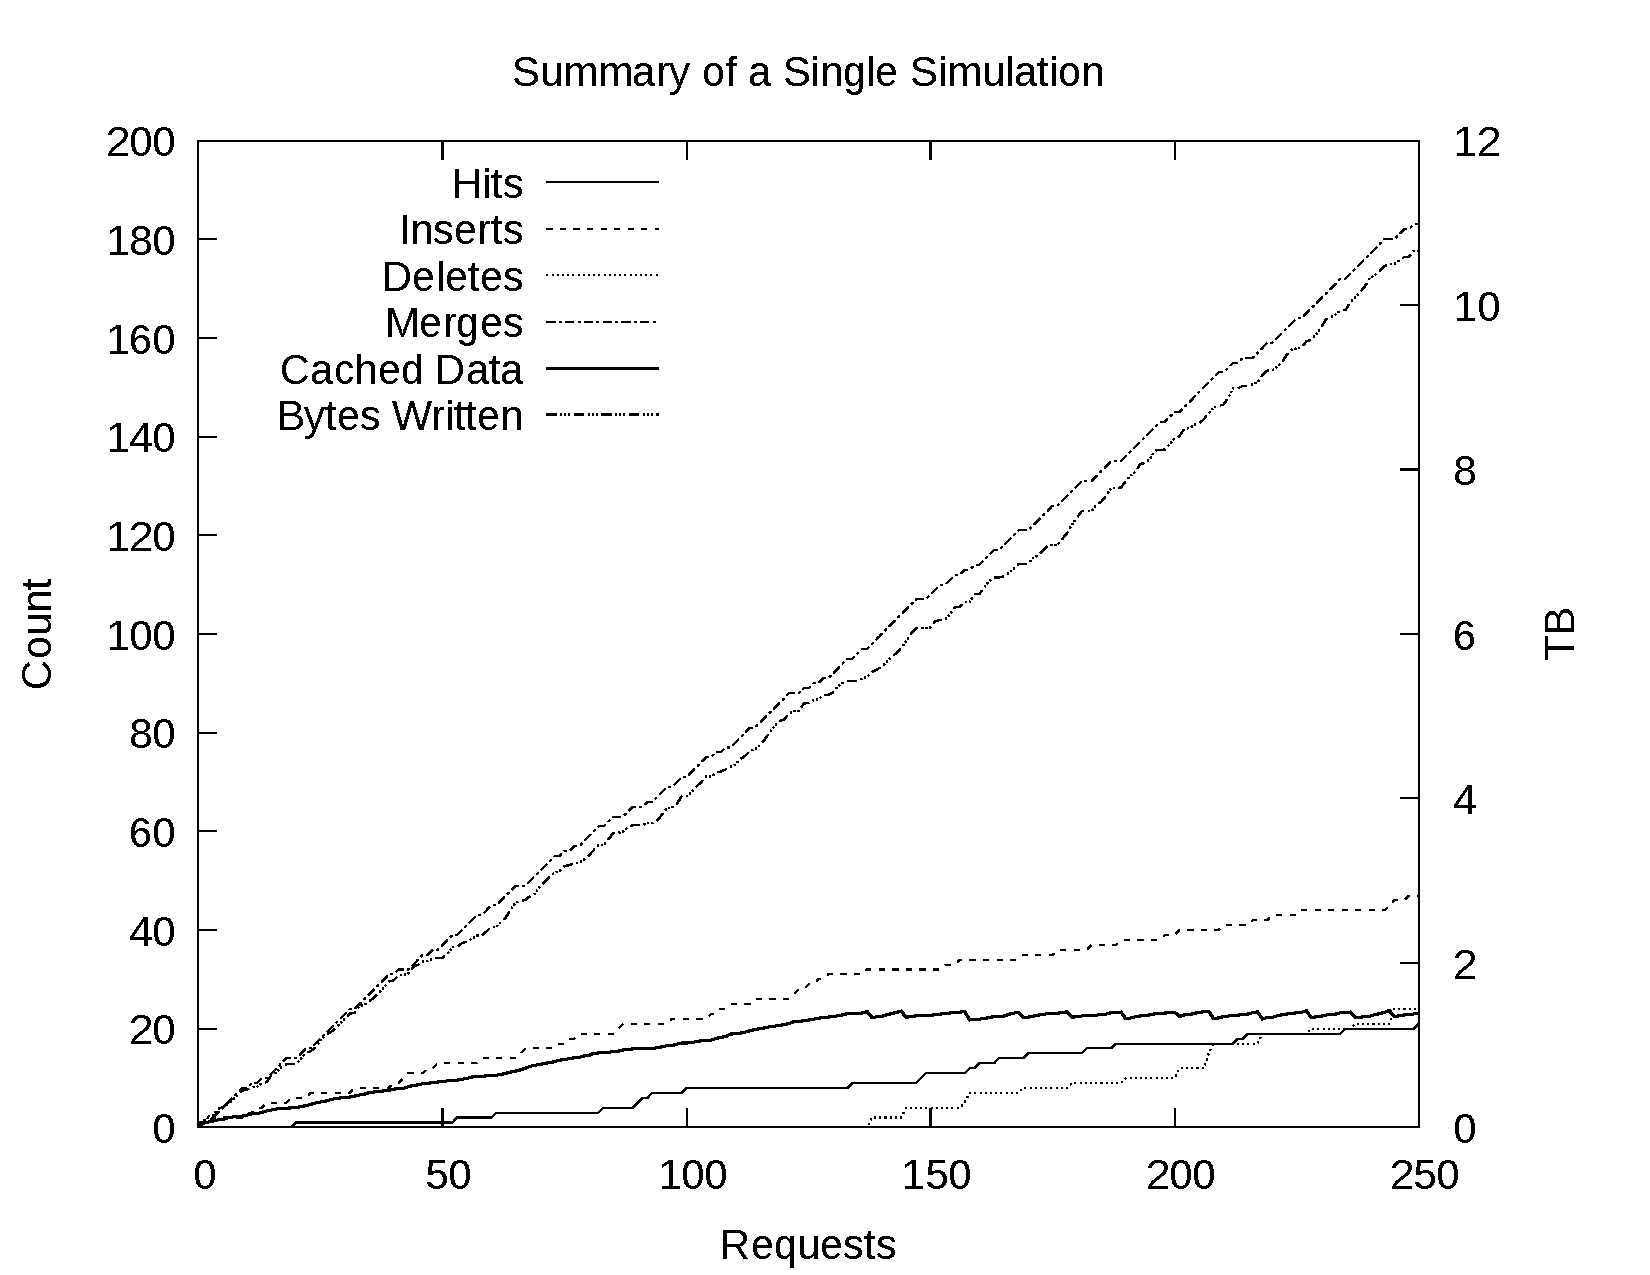
\includegraphics[width=\linewidth]{curated/time-series/time-series.pdf}
\caption{Behavior of a Single Simulation}
\label{fig:series}
\if 0
zoomed out?
cache limit, deletes start
merge tracks writes, it's the dominant factor
hits grow gradually as cache merges and fills
deletes help prune useless stuff, remaining should be frequent hits
far ends are either insert or merge, middle alphas have both
\fi
\end{figure}
    
\begin{figure}
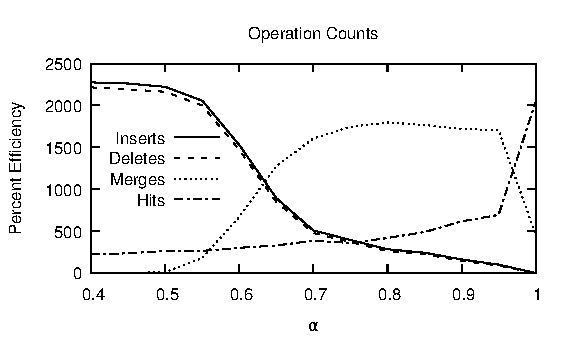
\includegraphics[width=\linewidth]{curated/comparative/operation_count.pdf}
\caption{Operation Counts for a Single Cache Configuration}
\label{fig:opcounts}
\if 0
inserts and merges switch as alpha goes up
more hits with merging
allows better responsiveness? image is immediately ready
inserts and deletes go to zero, so storage use will taper off
drop off: we keep everything, so 500 requests get merged; hit count goes up correspondingly since everything is in cache
not gonna be close to cache limit
inserts and deletes track: corresponds to LRU, inserts while filling then balanced
\fi
\end{figure}
    
    Figure~\ref{fig:series} shows a single simulation of our image management system
with $\alpha=0.0.75$ and cache size of 1.4~TB processing 500 unique job specifications, each one repeated five times.
First, we note that most of the operations are merges.
This is to be expected,
as this simulation ran with a fairly high $\alpha$ value.
The total bytes written also closely tracks merges,
indicating that merging is the dominant source of I/O.
We can still see inserts over the course of the simulation.
At more extreme $\alpha$ values,
we would expect to see one of these operations almost exclusively.
As the data in cache continues to rise,
we eventually see the cache limit,
after which the delete count starts increasing.
Over the course of the simulation,
inserts and deletes are filling and emptying the cache such that it remains close to its storage limit.
We also observe the number of cache hits continue to rise despite deletions.
As we will see, merging allows for a greater proportion of hits even if the amount of data remains constant.
This is because frequently used data can be merged,
reducing duplication.
The cache limit then ensures that infrequently used parts are eventually removed.

\section{Evaluation}
\label{sec:eval}

To evaluate the viability of our approach in automatically deduplicating a container image store,
we simulated the behavior of the system over time for a range of $\alpha$ values.
Choice of $\alpha$ is important here to ensure that common components can be detected and merged in container images,
and that old images or poor decisions are eventually removed from the system.
Choosing $\alpha$ too far in either direction will result in excessive storage overhead due to duplicated components,
or excessive compute and network overhead repeatedly merging largely unrelated images.
Our goal in this evaluation is therefore to choose $\alpha$ so as to minimize the storage and compute costs associated with maintaining a collection of images.


    %sweeping over alpha
    
    Since our simulation uses random simulated requests,
there is noticable variability between individual simulations.
Thus for a given choice of cache size, job count, etc.
we repeated the simulation 20 times and reported the median behavior over the runs.
At each choice of $\alpha$ (in steps of 0.05)
we performed a set of 20 simulated runs,
allowing us to plot various measurements of the system versus $\alpha$.

Sweeping over the range of $\alpha$ values in this way,
we can immediately see differences in the frequency of simulated operations.
Figure~\ref{fig:opcounts} shows the upper range of $\alpha$ values where behavior differences appear.
From the lower values on the left,
the insert and delete counts are the primary (or only) operations,
with number of hits relatively constant.
This corresponds to a simple LRU-based cache.
The insert count is higher due to cache filling,
but the two tend to increase in lockstep.
As $\alpha$ increases,
image merges become more probable.
The merge count in the figure steadily increases throughout most of the upper range,
while inserts and deletes decrease.
This suggests that at high $\alpha$ values,
the cache space would be more efficiently used,
with some of the duplication merged out.
In the extreme case with $\alpha=1$,
every request is merged into a single image in cache,
hence the sudden increase in hit rate and decrease in total merges at the far right of Figure~\ref{fig:opcounts}.
Note that as merging increases,
the proportion of hits generally also increases.
This indicates that more of the requests can be satisfied by previously merged images in the cache.
From the perspective of the system,
this is beneficial as there is no extra time or compute cost for handling a larger proportion of images.

    
\subsection{Measuring Efficiency of the System}

\begin{figure}
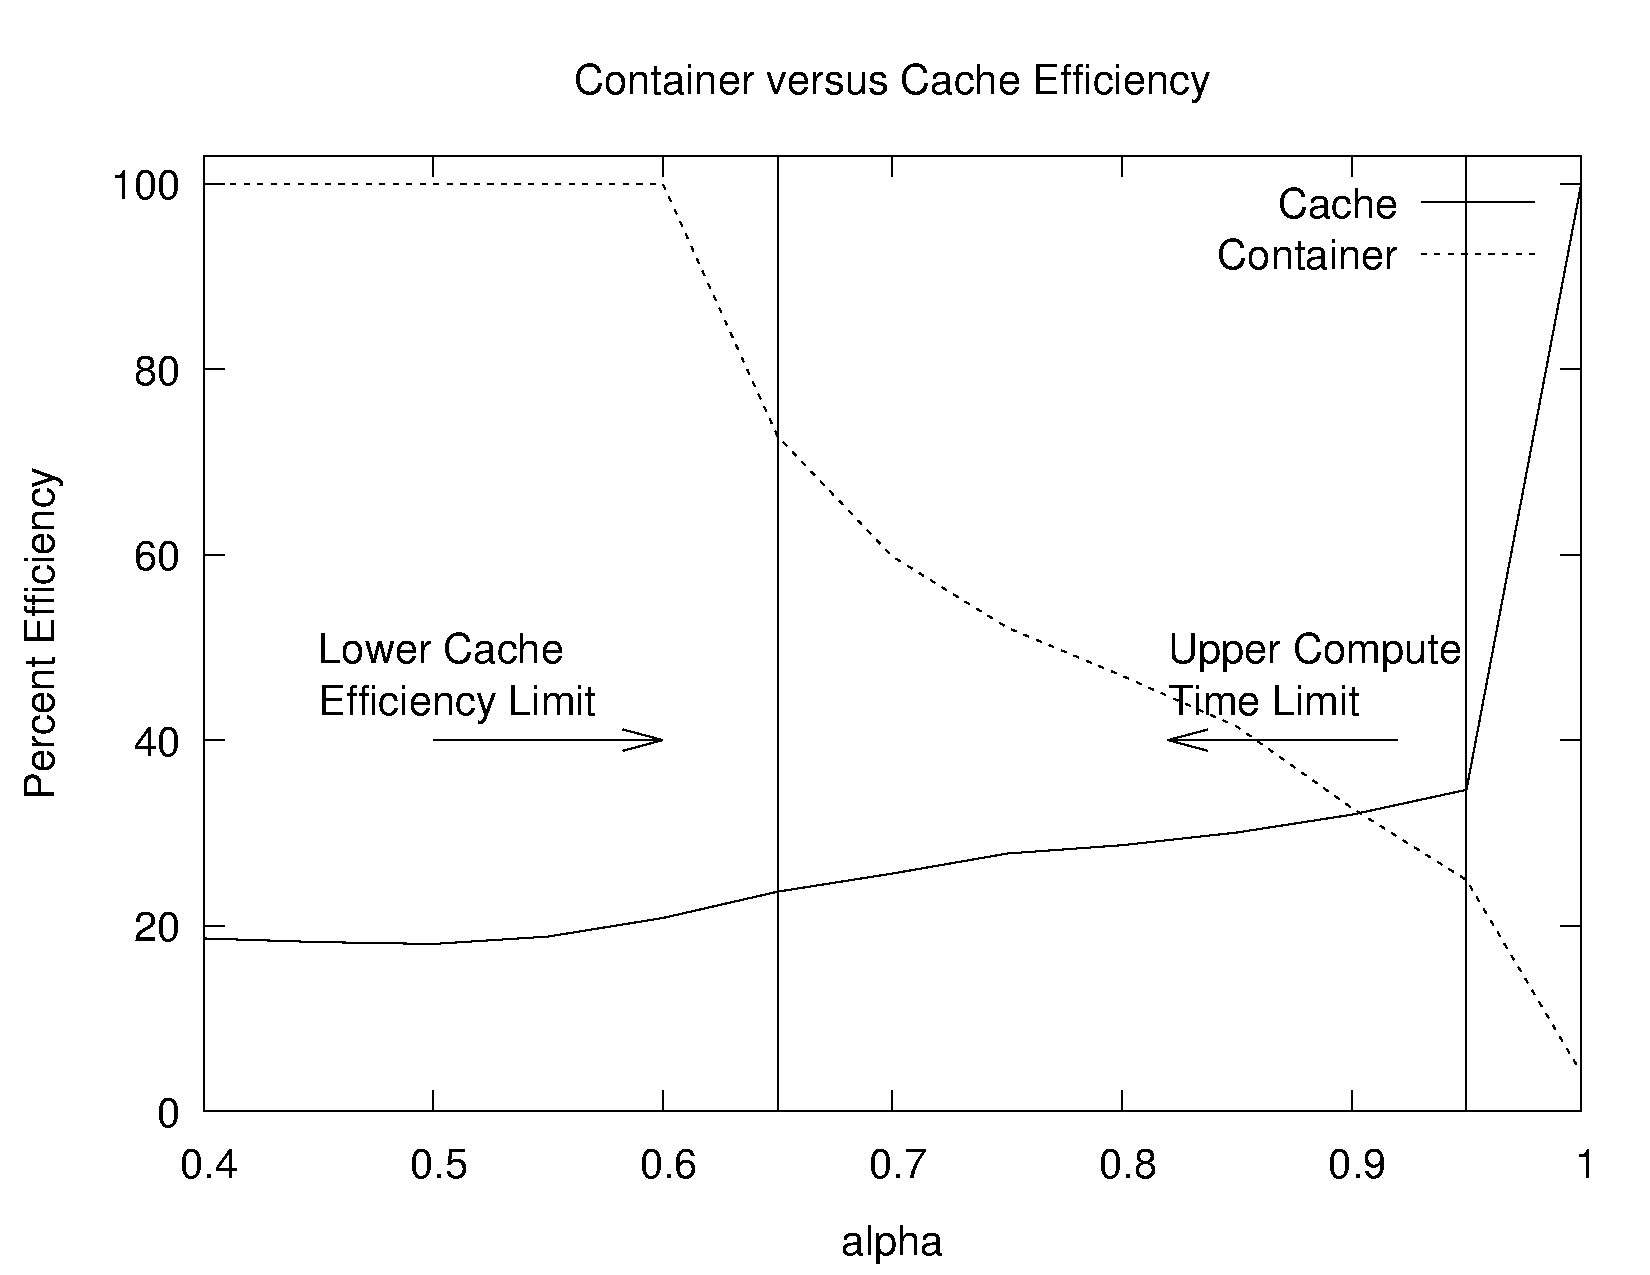
\includegraphics[width=\linewidth]{curated/comparative/distribution_efficiency.pdf}
\caption{Cache and Container Efficiency for a Representative Configuration}
\label{fig:dist-eff}
\if 0
explain what happened
metrics: why we care about efficiency?
cache efficiency: gauge duplication (waste), keeping working set costs lots of storage
container efficiency: unexpected overhead for each request; compute, network, etc.
place limits based on site, conditions
limits exist, we won't tell you
maybe just buy more cache?
large scale (10-100 TB), no can do...so need to merge sometimes
why 100 and 20 on the left
why they switch places: extreme cases
strike a balance
one curve might be more important for you
effects are not uniform/balanced gentle drop, massive spike in overhead on right
\fi
\end{figure}


\begin{figure}
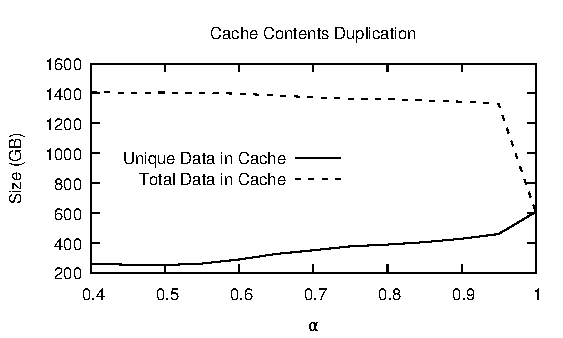
\includegraphics[width=\linewidth]{curated/comparative/cache_efficiency.pdf}
\caption{Duplication of Data in Cache}
\label{fig:cache-eff}
\if 0
justification for cache efficiency
unique vs total
full x range?
merging can give more unique data in less cache space
\fi
\end{figure}



\begin{figure}
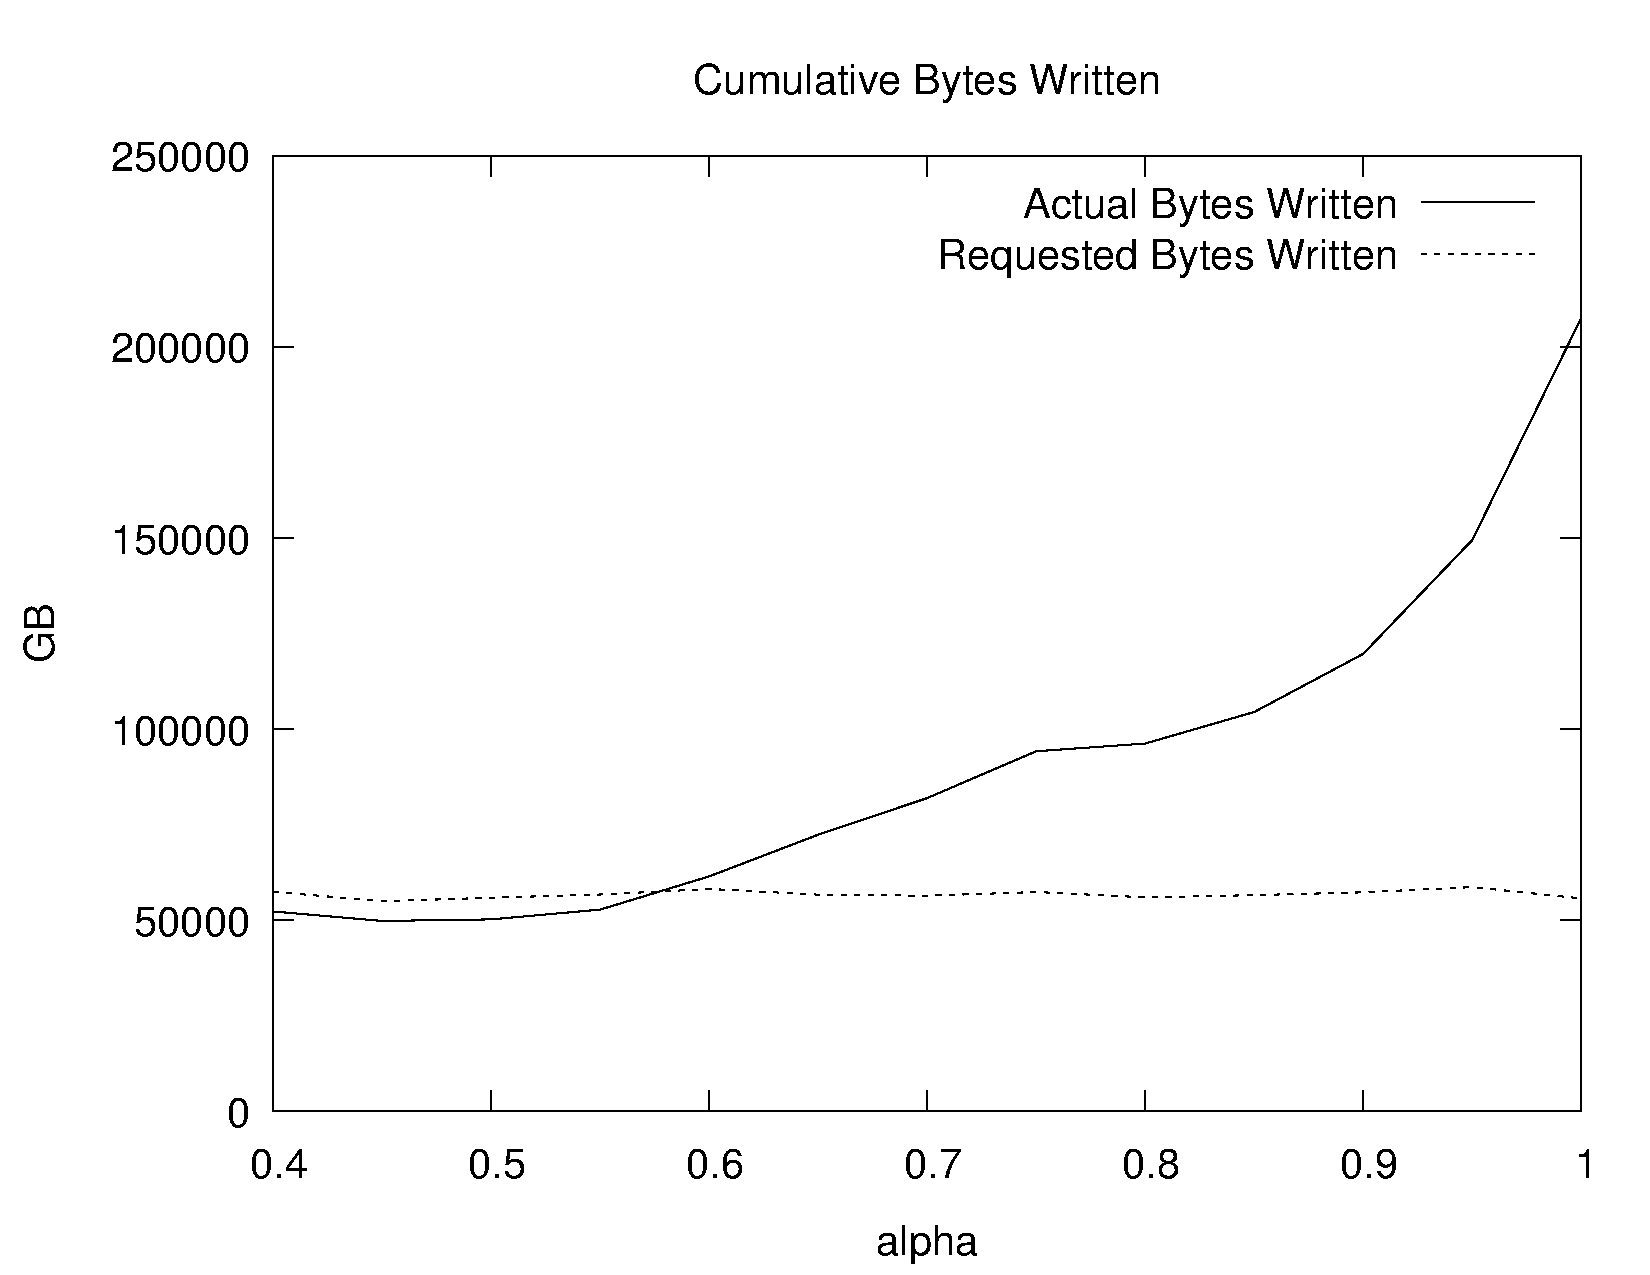
\includegraphics[width=\linewidth]{curated/comparative/container_efficiency.pdf}
\caption{Cumulative I/O Overhead}
\label{fig:container-eff}
\if 0
related to container efficiency: not exact but shows it
too much jitter from individual requests, so cumulative
crossover: hit rate allows reuse, so slightly less bytes written than requested
requested is based on random stream, constant
actual written goes up fast with alpha, so more overhead
proxy for compute/network/etc.
really steep at high alpha
\fi
\end{figure}


\begin{figure}
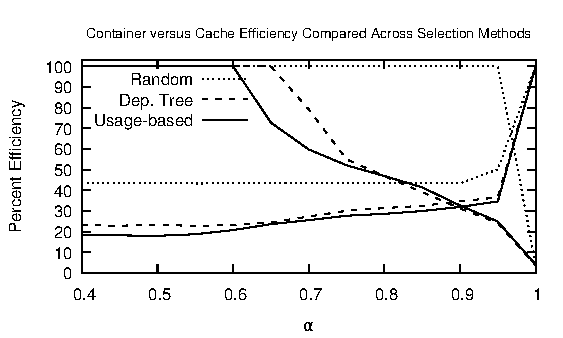
\includegraphics[width=\linewidth]{curated/comparative/distribution_efficiency_comp.pdf}
\caption{Efficiency Across Package Selection Methods}
\label{fig:comp-eff}
\if 0
different data patterns cause different effects
random has high utilization
pushed right, limited opportunity for merge, since no overlap
merging doesn't help
random is not realistic though
merging is not general solution, but for trees of software, look at this

tree has more duplication, starts merging much sooner
closure is very non-controvertial, but results in serious changes in efficiency
common to any software, so opportunity for optimization
common core that can merge to avoid dups
including usage stats (dist) amplifies these somewhat
real usage should be stronger than dist

use dist from now on because reasonable approximation to actual usage
similar to tree anyway
mild but noticable difference from tree, more natural approximation to real usage
\fi
\end{figure}

When sweeping over the range of $\alpha$ values,
there are a number of metrics available to summarize each simulation run.
Many, however, are highly coupled with the particular system configuration and difficult to compare as we vary the paramaters of the simulations.

We therefore chose to define two metrics, cache efficiency and container efficiency,
to indicate the relative utilization of the system.
Figure~\ref{fig:dist-eff} plots these two metrics for a representative simulation.
We defined cache efficiency as the ratio of unique data to total data in the cache.
In our case, this is equivalent to the ratio of the size of the unique packages to the total cache size.
If many images contain copies of the same packages,
the cache efficiency decreases.
This metric captures the extent of duplication within the cache across all images.
With no merging there is a high degree of duplication,
so the cache efficiency is low.
On the other end of the spectrum,
maintaining a single, large image containing all data results in cache efficiency of 100\%,
as the entire cache resides in that single image with no duplication

We defined container efficiency as the ratio of the size of the requested container
(in our case a set of requested packages plus all dependencies)
to the size of the container the system actually used for the job.
In the absence of merging,
these two are equal so the container efficiency is 100\%;
jobs are run with exactly what was requested.
By merging to allow for image reuse,
we include additional, unrequested data in container images.
The container efficiency measures this difference between requests and containers.
In the extreme case of $\alpha=1$ with a single large image, for example,
the container efficiency is poor because the entire repository is used for every request,
regardless of size.

These two extreme cases, no merging among many images and a single merged image,
can both be useful in some situations.
If the requirements of all jobs are known in advance and worker storage and bandwidth are sufficient,
maintaining a single, large image for all jobs on all workers is an useful strategy.
After the initial (costly) image creation and transfer,
there are no continuing costs or delays.
When resources are limited or requirements change regularly,
however, this approach becomes prohibitively expensive.
The high compute and bandwidth overhead apply for every image update,
which in the worst case could be every job.

The other extreme situation,
simply caching requests with no merging,
can also be viable.
This approach is simpler and does not come with extreme per-job overhead.
In addition, frequent changes to the jobs and requirements do not degrade the efficiency of each job.
At large scale, however,
the overall system efficiency suffers.
Due to duplication among images,
larger caches contain less and less unique data.
To support a given repository,
it can become necessary to provision a cache much larger than the size of the repository.
With common CVMFS repositories consuming several terabytes of storage each,
the amount of cache space grows quickly.

These two limiting factors,
the compute and transfer cost in the highly merged case and the cache efficiency in the unmerged case,
serve as limits on the viable range of $\alpha$ values for the system.
Figure~\ref{fig:dist-eff} shows two vertical lines indicating these limits on a plot of efficiencies.
The left line shows a lower limit of around 30\% on the cache efficiency.
Choosing $\alpha$ too low results in cache efficiency reaching below 20\%.
On the right, the line gives an upper limit on the likelihood of merging.
As shown in Figure~\ref{fig:opcounts},
the amount of I/O and compute to update images becomes much larger if $\alpha$ is set too high.
These two limits define a range of viable values for $\alpha$.
There is no general rule for the placement of these limits,
which depends strongly on the performance characteristics of the execution environment,
as well as the priorities of the administrators in optimizing the system.
Rather than defining where these limits fall,
we give per-site considerations in choosing limits in Section~\ref{ANALYSIS_SECTION}.

Figure~\ref{fig:cache-eff} shows the actual data sizes used to calculate the cache efficiency.
Without merging, the unique data makes up a small proportion of the cache.
With increased merging, the amount of unique data increases.
For sufficiently high $\alpha$,
merges occur more frequently than cache inserts,
resulting a drop in total storage size.
On the far right of Figure~\ref{fig:cache-eff},
the entire cache contents are merged into a single large image,
so that the unique and total data sizes become equal.
The cache efficiency metric is affected both by the increase in unique data and by the decrease in total cache size.

Figure~\ref{fig:container-eff} shows the cumulative costs of creating and updating images relative to the cost of simply providing the requested images.
These costs illustrate the effect of container efficiency over the course of a simulated run.
Without merging, the actual I/O and compute costs in the system closely follow the requests.
In Figure~\ref{fig:container-eff} the actual I/O is slightly smaller than the requested amount due to caching:
the system can sometimes reuse images without performing any I/O.
As $\alpha$ increases, the cost of updating and merging images comes to dominate the total cost.
Administrators migh decide, for example,
to spend at most twice the compute and I/O time relative to the the actual requested operations.
This would correspond to the upper compute limit shown on \Cref{fig:dist-eff}.
Depending on the priorities at a particular execution site,
either the storage utilization or compute and I/O time could be the critical factor in optimizing performance.

\begin{figure*}[ht]
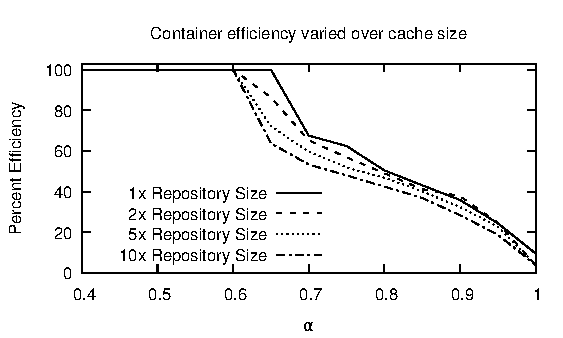
\includegraphics[width=0.48\linewidth]{curated/sensitivity/container_efficiency_cache.pdf}
\hfill
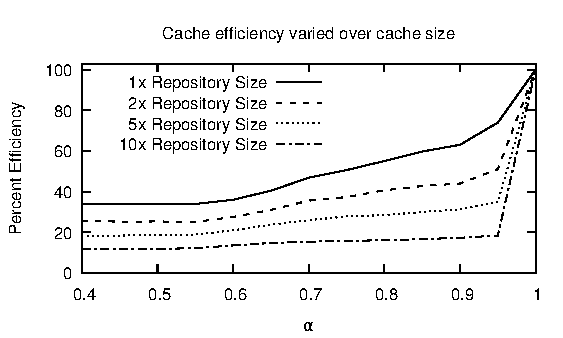
\includegraphics[width=0.48\linewidth]{curated/sensitivity/cache_efficiency_cache.pdf}
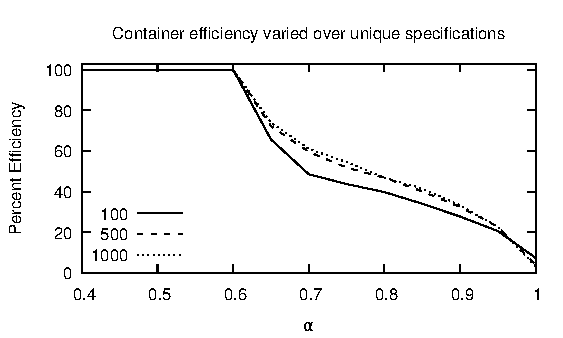
\includegraphics[width=0.48\linewidth]{curated/sensitivity/container_efficiency_request.pdf}
\hfill
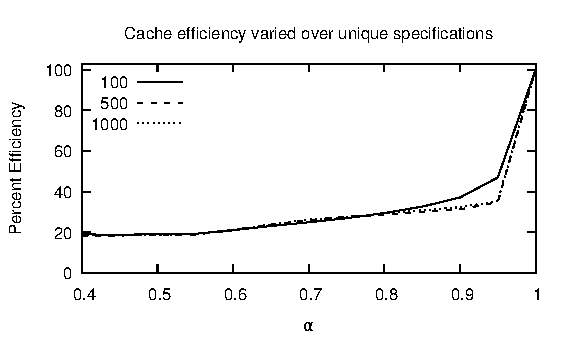
\includegraphics[width=0.48\linewidth]{curated/sensitivity/cache_efficiency_request.pdf}
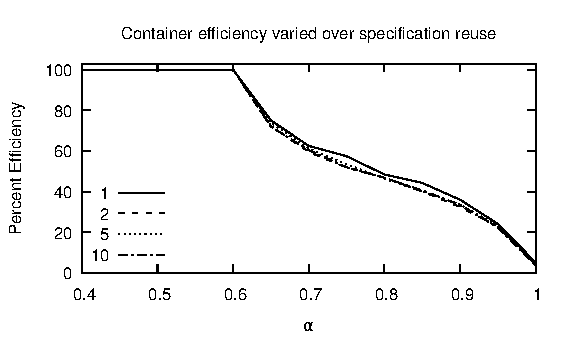
\includegraphics[width=0.48\linewidth]{curated/sensitivity/container_efficiency_uses.pdf}
\hfill
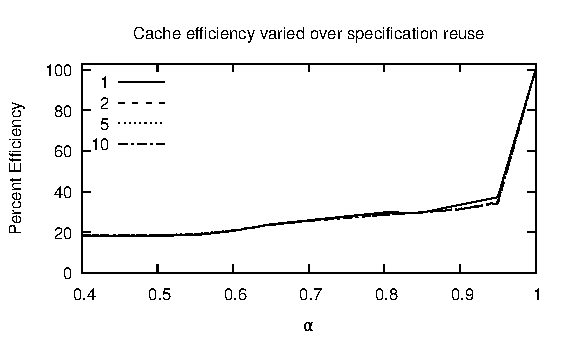
\includegraphics[width=0.48\linewidth]{curated/sensitivity/cache_efficiency_uses.pdf}
\caption{Effects of Simulation Parameters on System Efficiency}
\label{fig:sensitivity}
\if 0
[t] "just buy more cache"
efficiency is worse, since cache holds on to lots of questionable data
loads of opportunities to try merges, so we see a lot of unnecessary merges
less force removing bad choices, so more cruft can accumulate in many images
better cache utilization with tiny cache, but of course more thrashing
at scale, bad idea
large cache is too pricey at scale
[m] varying reuse doesn't affect too much
below 100 doesn't seem full/steady state yet
cache isn't settled? so haven't dropped bad merges; more unique data in cache boosts efficiency
[b] high number of requests, repeats don't matter
unique data dominates
hard to tell difference between [m] and [b], so not too sensitive to these
once you hit steady state, jobs count/repeats has little effect on efficiency
general trends of merging, not interesting by themselves
\fi
\end{figure*}    

\subsection{Comparison of Simulated Image Types}

We also compared the efficiencies of several types simulated images under a range of $\alpha$ values.
For the previous discussion, synthetic images were generated taking into account both the tree of package dependencies and usage statistics.
Figure~\ref{fig:comp-eff} shows a representative simulation with two other synthetic image types included.
First, we measured images considering only the dependency relationships but not usage.
These images show similar behavior to those previously discussed,
albeit with slightly lower efficiencies.
More realistic images primarily make the same trends more pronounced.
This suggests that even with random, non-realistic requests,
the tree structure of package dependencies is sufficient to produce duplication in the cache.
The other type of synthetic image shown in Figure~\ref{fig:comp-eff} is purely randomly generated.
The set of packages in each image was chosen uniformly randomly from the full SFT repository.
These random images do not take into account usage statistics or package dependencies,
making the software in them entirely nonfunctional.
For the random images,
we observe markedly different cache behavior.
The cache efficiency is much higher,
indicating a greater proportion of unique data in the cache.
Since the image contents were selected purely at random,
this is expected.
The container efficiency is also high over a much larger range of $\alpha$ values.
This is because there is effectively no merging until extremely high $\alpha$.
Since image contents are purely random,
there is no correlation between different images.
Thus, it is much more difficult to find images similar enough to merge until the $\alpha$ value is very lax.
This would indicate that our merging strategy is not applicable to arbitrary collections of data.
Random images show little to no effect for most $\alpha$ values.
Our merging strategy, which takes advantage of duplicated content included as a result of dependencies in software,
would be ill advised for situations that are not known to follow similar patterns of duplication.

\subsection{Sensitivity Analysis}
\label{sec:sensitivity}

    
    In Figure~\Cref{fig:sensitivity}, we plot efficiency curves for a range of simulation conditions.
The left column shows container efficiency,
while the right column shows cache efficiency.
In the first row, the number of jobs and the amount of repetition are constant while the cache size is varied.
In the second row, the number of unique requests is varied with the other parameters constant,
and the third row varies the number of times each job is submitted with the rest constant.

The size of the cache has an inverse relationship with both the container and cache efficiency.
A larger cache can of course hold a larger number of images,
but since each image contains significant duplicated portions,
increasing cache size tends to decrease cache efficiency.
Conversely, small caches more quickly evict images so that ineffective merges and similar images tend not to remain in cache too long.
A larger cache also allows for more opportunities to merge images,
leading to decreased container efficiency.
When deciding how to handle a request,
a large cache full of images is much more likely to contain an image suitable for merging.
With a small cache, opportunities to merge are much more dependent on the order in which requests happen to come.

The effect of varying the number of unique jobs is less pronounced than the effect of cache size.
Streams of 500 and 1000 unique jobs show nearly indistinguishable behavior,
indicating that by 500 jobs the system has reached a steady state.
Continuing with an arbitrarily long stream should not result in significant performance changes.
It appears that 100 unique jobs were not sufficient to fill the cache and reach a steady state.
In this case the container efficiency is slightly decreased over $\alpha$,
suggesting that some ineffective merges had not made their way out of the cache yet.
The cache efficiency in this case is slightly increased.
This would suggest that before reaching a steady state,
the cache contents are more assorted and some unnecessary data remains cached.

The effect of varying the number of times each unique job is submitted appear minimal at best.
As discussed with the previous row,
a stream of 500 unique images should be sufficient to reach a steady state.
For a sufficiently large cache, therefore,
it appears that the efficiency is determined by the amount of unique data and fairly insensitive to how much those pieces of data are used.
This simulation is somewhat unrealistic in that each job is repeated a uniform number of times.
In real systems, we expect more variation in the frequency of repeated jobs.
We predict that a steady, non-uniform distribution of frequencies would result in the same behavior as shown in the bottom row of Figure~\ref{fig:sensitivity},
while changes in the frequencies of jobs (e.g. a new user starting an experiment)
would disturb the steady state and produce effects similar to those in the middle row.
    
\subsection{Choosing $\alpha$ Threshold}
\label{ANALYSIS_SECTION}

Based on the previous analyses of simulated cache behavior,
some trends emerge in the effect of choice of $\alpha$ with varying cache parameters.
While there is no general rule for applying our approach to real sites,
these trends give some guidance.
The absolute simplest method to improve caching behavior is not to merge images and to increase the size of the cache.
For a small number of users or infrequent changes to containers,
this might be all that is needed.
At the scale under consideration here, however,
this somewhat tongue-in-cheek advice easily becomes unfeasible.
As shown in \Cref{fig:sensitivity},
the cache efficiency without merging often falls below 20\%.
When working with one or more repositories containing several terabytes of data each,
provisioning a cache large enough to hold highly duplicated images becomes expensive.
This storage cost gives a lower limit in choosing $\alpha$.
Rather than committing tens of terabytes to a cache,
sites may prefer to devote a larger proportion of compute and network bandwidth to image management.
Since the compute overhead grows very quickly at high $\alpha$,
it would be ill advised to push this value too high.
The safer approach to choosing $\alpha$ is to start at the lower limit and gradually increase $\alpha$,
observing the changes in compute overhead.


%%%%%%%%%%%%%%%%%%%%
\if 0
where software is provided as needed in the form of RPM files or another similar format.
Working with software packages is simpler in that dependencies are explicitly specified in the package file or database.
With CVMFS, no such definitive specification exists.
This issue is common to shared/global filesystems,
since users expect the complete contents to be available on demand and so devote little time to explicitly defining dependencies and other requirements.

CVMFS differs from traditional POSIX filesystems in that previous versions of all content remain available.
A researcher may specify the precise revision under which an application is known to run.
Thus the same path may refer to two completely different files for a pair of applications.
This is beneficial from the standpoint of reliability and reproducibility,
but complicates the process of projection.
A file specification needs to include enough information
to establish the directory structure and verify the contents at a specific revision.
This can be done in several ways, 
such as computing the checksum of contents,
using global revision numbers, 
or running verification software.
Computed checksums provide a system agnostic approach
to verification by allowing the checksum to be computed
at specification and verified before use.
Computed checksums provide a
consistency guarantee to the byte level,
but are often expensive at runtime for large
production systems.
This approach is alleviated in systems such as 
Git and CVMFS as the contents' checksums are 
computed at ingestion into the repository.
This method relies on the underlying system computing
and providing this information for verification.
\fi


\section{Related Work}
\subsection{Container Technology}
A core assumption presented in this paper is that 
container technology is relied on for packaging and
transporting the projections to the compute site.
Unfortunately, which of a variety of solution is used 
depends on the actual site.
Currently, the most popular solutions are
Docker\cite{Merkel:2014:DLL:2600239.2600241} and
Singularity\cite{Singularity}.
Docker is more ubiquitous, but its 
obfuscated implementation and privileged user requirements 
are leading more scientist and site administrator
to Singularity.
Additionally, site often spin-off highly tailored implementation
like Shifter\cite{Jacobsen2015ContainT} at NERSC
and Slacker\cite{194430}, which provide slim containers
for moving around that bootstrap larger systems.

In recent years, with the announcement of user namespaces
and unprivileged filesystem mounts~\cite{user-filesys-mount}, notably FUSE, 
containers, image formats, and different environment specification
use will increase and proliferate increasing the need for a container
agnostic approach until more consistency is reached.
This will likely lead to more simplified container implements such as
CharlieCloud\cite{Priedhorsky:2017:CUC:3126908.3126925}.


\section{Conclusion}

Global filesystems offer a convenient way to organize and distribute the large, complex, and frequently updated software repositories that support international scientific experiment collaborations such as ATLAS, CMS, LIGO, and LSST.
The software in these repositories consists of millions of files and terabytes of data.
The massive scale of these projects would not be possible without software such as CVMFS to ensure consistency and availability of software at sites across the globe.
At some computing facilities, especially national HPC sites,
restrictions on the worker activity and network access make global filesystem access difficult or impossible.
To take advantage of local high performance filesystems and container technologies available at such sites,
we introduced the concept of projecting subsets of the global filesystem into local resources.
We instrumented CVMFS to add support for tracing application dependencies,
and developed a tool for efficiently projecting CVMFS into local container images suitable for use at HPC facilities.
When working with many users and at large scale, however,
the straightforward approaches to managing these projected images fall short.
We proposed a simple strategy for managing a cache of projected images,
taking advantage of usage patterns and duplication of software collections to reduce data duplication among containers.
Our approach allows users or system administrators to balance the storage cost associated with small, tailored container images against the computational and bandwidth costs of maintaining large, multi-job images.
Using our cache management approach,
applications can continue to take advantage of precise dependency requirements,
while users and administrators can fit performance and storage costs to meet the requirements of their particular execution sites.

\if 0
\section{Reproducibility Data}

In an effort to provide consistent, reproducible results outlined are the
resources utilized in this paper and where they can be found.
Specific commits are mentioned to provide the exact version that was used.


All of these repositories are open source and contain Makefiles
and instructions on how to build and run them.
\fi

%\section*{Acknowledgment}


\bibliographystyle{ACM-Reference-Format}
\bibliography{otherpapers,cclpapers}

\end{document}
